
%%%%%%%%%%%%%%%%                                ~~~~~~~~~~~~~~~~~~~~~~~~~~~~~~~~~~~~~~~~~~~~~~~~~~
% CONDITIONALS %
%%%%%%%%%%%%%%%%                                ~~~~~~~~~~~~~~~~~~~~~~~~~~~~~~~~~~~~~~~~~~~~~~~~~~

\newif\ifPeerReview\PeerReviewfalse             % Whether to create the PeerReview version or
                                                % Journal version
\newif\ifFlatArchive\FlatArchivefalse           % Whether archive is flat (messy) or contain 
                                                % subfolders for graphics etc.
\newif\ifFloatAtEnd\FloatAtEndfalse             % Available in PeerReview mode:
                                                % Place floats at end of document?
\newif\ifTODO\TODOtrue                        % Use todo notes?

%%%%%%%%%%%%                                    ~~~~~~~~~~~~~~~~~~~~~~~~~~~~~~~~~~~~~~~~~~~~~~~~~~
% IEEEtran %
%%%%%%%%%%%%                                    ~~~~~~~~~~~~~~~~~~~~~~~~~~~~~~~~~~~~~~~~~~~~~~~~~~

\ifPeerReview
\documentclass[12pt,journal,captionsoff,onecolumn,english]{IEEEtran}
\newcommand\CLASSINPUTbaselinestretch{1.66}     % http://theoval.cmp.uea.ac.uk/~nlct/latex/thesis/node17.html
\else
\documentclass[journal]{IEEEtran}
\fi



%%%%%%%%%%%%%%%%%%%%%%%%%%%%%%                  ~~~~~~~~~~~~~~~~~~~~~~~~~~~~~~~~~~~~~~~~~~~~~~~~~~
% IEEE ''APPROVED'' PACKAGES %
%%%%%%%%%%%%%%%%%%%%%%%%%%%%%%                  ~~~~~~~~~~~~~~~~~~~~~~~~~~~~~~~~~~~~~~~~~~~~~~~~~~


\ifCLASSINFOpdf
   \usepackage[dvips]{graphicx}                 % Might not work. Use 'latex' instead of 
   \ifFlatArchive\else                          % 'pdflatex'
      \graphicspath{./gfx/}
   \fi
\else
   \usepackage[dvips]{graphicx}
   \ifFlatArchive\else
      \graphicspath{./gfx/}
   \fi
\fi

\RequirePackage[table,dvipsnames,svgnames]{xcolor}

\usepackage[cmex10]{amsmath}                    % cmex10 option to be IEEE explore compliant
\interdisplaylinepenalty=2500                   % Allows multiline equations to be broken

% \RequirePackage{amssymb}

\RequirePackage{array}

\ifCLASSOPTIONcompsoc
   \usepackage[caption=false,font=normalsize,labelfont=sf,textfont=sf]{subfig}
\else
   \usepackage[caption=false,font=footnotesize]{subfig}
\fi
\ifCLASSOPTIONcaptionsoff                       % IEEE promoted hack to turn off captions from the 
   \let\MYorigsubfloat\subfloat                 % subfloat package should the captionsoff option
   \renewcommand{\subfloat}[2][\relax]{\MYorigsubfloat[]{#2}} % be specified.
\fi

\ifFloatAtEnd
\ifCLASSOPTIONcaptionsoff                       % Places float at the end of the document when the
  \usepackage[nomarkers]{endfloat}              % captionsoff options is specified to IEEEtrans.cls
  \let\MYoriglatexcaption\caption               % (PeerReview mode)
  \renewcommand{\caption}[2][\relax]{\MYoriglatexcaption[#2]{#2}}
\fi
\fi

\usepackage{fixltx2e}                           % Fix some twocolumn float problems

%\usepackage{stfloats}                          % Allows: \begin{figure*}[!b]
                                                % (double column figures on top/bottom)

\usepackage{url}                                % Support for handling and breaking URLs

% NOTE: PDF hyperlink and bookmark features are not required in IEEE
%       papers and their use requires extra complexity and work.
\newcommand\MYhyperrefoptions{bookmarks=true,bookmarksnumbered=true,
pdfpagemode={UseOutlines},plainpages=false,pdfpagelabels=true,
colorlinks=true,linkcolor={black},citecolor={black},urlcolor={black},
pdftitle={Low Complexity Adaptive Beamformer for Active Sonar Imaging},
pdfsubject={},
pdfauthor={Jo Inge Buskenes},
pdfkeywords={adaptive beamforming, beamforming, complexity, sonar, active}}%
\ifCLASSINFOpdf
   \usepackage[\MYhyperrefoptions,pdftex]{hyperref}
\else
   \usepackage[\MYhyperrefoptions,breaklinks=true,dvips]{hyperref}
   \usepackage{breakurl}                        % Allows 'dvips' driver to break links
\fi

%%%%%%%%%%%%%%%%%%%%%%%                         ~~~~~~~~~~~~~~~~~~~~~~~~~~~~~~~~~~~~~~~~~~~~~~~~~~
% ADDITIONAL PACKAGES %       
%%%%%%%%%%%%%%%%%%%%%%%                         ~~~~~~~~~~~~~~~~~~~~~~~~~~~~~~~~~~~~~~~~~~~~~~~~~~

\usepackage[maxfloats=25]{morefloats}
\newcounter{todoidx}
% \setcounter{todoidx}

\ifTODO
   \definecolor{todobackground}{rgb}{0.95,0.95,0.95}
   \setlength\marginparsep{1pt}
   \setlength\marginparwidth{35pt}
   \newlength\marginparwidthsmall
   \setlength\marginparwidthsmall{\marginparwidth}
   \addtolength\marginparwidthsmall{-7pt}
   \newcommand\todo[1]{%
      \addtocounter{todoidx}{1}%
      {\color{Red}\fbox{\bf\thetodoidx{}}}%
      \marginpar{%
         {\vspace*{-10pt}\color{Red}\fbox{\bf\thetodoidx{}}}\\%
         \fcolorbox{red}{todobackground}{\parbox{\marginparwidthsmall}{\scriptsize #1}}}}

   \newcommand\todopar[1]{\fcolorbox{red}{white}{\parbox{0.97\linewidth}{#1}}}
\else
%    \usepackage[disable]{./todonotes} 
   \newcommand\todo[1]{}
\fi

\newenvironment{narrow}[2]{%
\begin{list}{}{%
\setlength{\topsep}{0pt}%
\setlength{\leftmargin}{#1}%
\setlength{\rightmargin}{#2}%
\setlength{\listparindent}{\parindent}%
\setlength{\itemindent}{\parindent}%
\setlength{\parsep}{\parskip}}%
\item[]}{\end{list}}


%%%%%%%%%%                                      ~~~~~~~~~~~~~~~~~~~~~~~~~~~~~~~~~~~~~~~~~~~~~~~~~~
% MACROS %       
%%%%%%%%%%                                      ~~~~~~~~~~~~~~~~~~~~~~~~~~~~~~~~~~~~~~~~~~~~~~~~~~


\newcommand\Grey[1]{{\color{Grey}#1}}
\newcommand\Red[1]{{\color{Red}#1}}
\newcommand\Blue[1]{{\color{Blue}#1}}
\newcommand\DarkBlue[1]{{\color{DarkBlue}#1}}
\newcommand\LightBlue[1]{{\color{LightBlue}#1}}
\newcommand\Brown[1]{{\color{Brown}#1}}
\newcommand\Green[1]{{\color{Green}#1}}
\newcommand\SeaGreen[1]{{\color{SeaGreen}#1}}
\newcommand\Yellow[1]{{\color{yellow}#1}}
\newcommand\Orange[1]{{\color{orange}#1}}

\newcommand\nn{\nonumber\\}

\newcommand\nmat[1]{\begin{matrix}#1\end{matrix}}
\newcommand\bmat[1]{\begin{bmatrix}#1\end{bmatrix}}
\newcommand\case[1]{\begin{cases}#1\end{cases}}
\newcommand\textbox[2]{\footnotesize\text{\parbox{#1}{\centering\emph{#2}}}}

\newcommand\rand{\text{rand}}
\newcommand\randn{\text{randn}}
\newcommand\rect{\text{rect}}
\newcommand\sinc{\text{sinc}}
\newcommand\tr{\text{tr}}
\newcommand\adj{\text{adj}}

% \newcommand\max{\text{max}}
\newcommand\argmin{\text{argmin}}

\newcommand\qqquad{\quad\qquad}
\newcommand\qqqquad{\qquad\qquad}

\renewcommand\l[1]{\left#1}
\renewcommand\r[1]{\right#1}

% {\text{\parbox{1.5cm}{\centering volume hyper- sphere}}}

%Keyword colouring:
\newcommand\kw[1]{#1}
\newcommand\parm[1]{#1}%\color{Black}#1\color{Black}}

\newcommand\of[1]{\scriptstyle(\parm{#1})\displaystyle}
\newcommand\df[1]{\scriptstyle[\parm{#1}]\displaystyle}
\newcommand\var[3]{#1_\text{#2}\of{#3}}

\newcommand\diag{\text{diag}}

% \raisebox{lift}[extend-above-baseline][extend-below-baseline]{text}
\newcommand\mt[1]{\text{\emph{#1}}} %mt = mathtext
\newcommand\mathnorm{\textstyle}
\newcommand\mathbig[1]{\displaystyle#1\mathnorm}
\newcommand\mathsmall[1]{\scriptstyle#1\mathnorm}
\newcommand\mathtiny[1]{\scriptscriptstyle#1\mathnorm}
\newcommand\sfrac[2]{\scriptstyle\raisebox{0.25pt}[0pt][0pt]{$\frac{#1}{#2}$}\mathnorm}
\newcommand\nfrac[2]{\textstyle\frac{#1}{#2}\displaystyle}

\newcommand\sumu[1]{\sum\limits^{#1}\,}
\newcommand\suml[1]{\sum\limits_{#1}\,}
\newcommand\sumb[2]{\sum\limits_{#1}^{#2}\,}

\newcommand\produ[1]{\prod\limits^{#1}\,}
\newcommand\prodl[1]{\prod\limits_{#1}\,}
\newcommand\prodb[2]{\prod\limits_{#1}^{#2}\,}

%Math macros:
\newcommand\diff[2]{\frac{\kw{d}\,\textstyle #1\scriptstyle}{\kw{d\parm{#2}}}\displaystyle}
\newcommand\ddiff[2]{\frac{\kw{d^2}\,\displaystyle #1\scriptstyle}{\kw{d\parm{#2}}^2}\displaystyle}

\renewcommand\d[1]{\scriptstyle\kw{\,d\parm{#1}}\displaystyle}

% These commands are mutually exclusive. Remember to "renew" in v2.
\newcommand\intb[4]{\int\limits_{#3}^{#4} #1 \d{#2}} % \int{exp}{var}{from}{to}
\newcommand\intl[3]{\int\limits_{#3} #1 \d{#2}} % \int{exp}{var}{for all}
\newcommand\intu[2]{\int #1 \d{#2}} % \int{exp}{var}{for all}

\newcommand\T{^{\scriptscriptstyle T}}
\renewcommand\H{^{\scriptscriptstyle H}}

\renewcommand\vec[1]{\boldsymbol{#1}}
\newcommand\mat[1]{\boldsymbol{#1}}


\renewcommand*\a{\vec a}
\renewcommand*\i{\vec i}
\renewcommand*\k{\vec k}
\newcommand*\n{\vec n}
\newcommand*\p{\vec p}
\newcommand*\s{\vec s}
\newcommand*\w{\vec w}
\newcommand*\x{\vec x}
\newcommand*\y{\vec y}

\newcommand*\A{\mat A}
\newcommand*\B{\mat B}
\newcommand*\C{\mat C}
\newcommand*\E{\mat E}
% \renewcommand*\H{\mat H}
\renewcommand*\P{\mat P}
\newcommand*\eP{\mat{\hat P}}
\newcommand*\R{\mat R}
\newcommand*\Ri{\R^{-1}}
\newcommand*\eR{\mat{\hat R}}
\newcommand*\W{\mat W}
\newcommand*\X{\mat X}
\newcommand*\Xd{\X_{\!\Delta}}
\newcommand*\Y{\mat Y}

\renewcommand*\L{\mat \Lambda}
\newcommand*\U{\mat U}
% \renewcommand*\t{\mathtiny{^T}}
% \newcommand*\h{\mathtiny{^H}}
\renewcommand*\t{^T}
\newcommand*\h{^H}

\newcommand\D{\vec\nabla} %Del: Vector differential operator - nabla
\newcommand\Dx{\vec\nabla\times}
\newcommand\Dd{\vec\nabla\cdot}

\usepackage{tikz}
\usetikzlibrary{shapes,snakes}
\usepackage{amsmath,amssymb}

\newenvironment{outline}
{\begin{itemize}}
{\end{itemize}}

%    \definecolor{todobackground}{rgb}{0.95,0.95,0.95}
%    \setlength\marginparsep{3pt}
%    \setlength\marginparwidth{42pt}
%    \newlength\marginparwidthsmall
%    \setlength\marginparwidthsmall{\marginparwidth}
%    \addtolength\marginparwidthsmall{-7pt}
%    \newcommand\todo[1]{%
%       \addtocounter{todoidx}{1}%
%       {\color{Red}\fbox{\bf\thetodoidx{}}}%
%       \marginpar{%
%          {\vspace*{-10pt}\color{Red}\fbox{\bf\thetodoidx{}}}\\%
%          \fcolorbox{red}{todobackground}{\parbox{\marginparwidthsmall}{#1}}}}
% 

% correct bad hyphenation here
% \hyphenation{op-tical net-works semi-conduc-tor}


%%%%%%%%%%%%%%%%%%                              ~~~~~~~~~~~~~~~~~~~~~~~~~~~~~~~~~~~~~~~~~~~~~~~~~~
% DOCUMENT START %
%%%%%%%%%%%%%%%%%%                              ~~~~~~~~~~~~~~~~~~~~~~~~~~~~~~~~~~~~~~~~~~~~~~~~~~

% \RequirePackage[utf8]{inputenc}%              % Set input encoding (optionally latin1)
% \RequirePackage[T1]{fontenc}%                 % Set font encoding


\begin{document}

\newpage
\begin{figure*}[!t]
\begin{narrow}{-1.2cm}{-1.2cm}\centering\vspace{-1.0cm}
\textbf{1. LCA with trigonometric and Kaiser windows - Capon shining}\\
\begin{tabular}[c]{l l l l}
\bf General & M = 32                            & $\Delta r = \frac{c}{2B}$ = 2.5 cm & $\frac{640\,\text{pixels}] / 12\,\text{m}}{\Delta r} = \frac{4}{3}$ \\
\bf LCA     & $\beta \in [0,10]$ (9 values) & $\phi \in [-1.07,1.07]$ deg (9 values) & Navg = 3 \\
\bf Capon   & $\Delta$ = 0.01                 & L = 16                           & Navg = 3 \\
\end{tabular}
\subfloat[LCA Window Response]{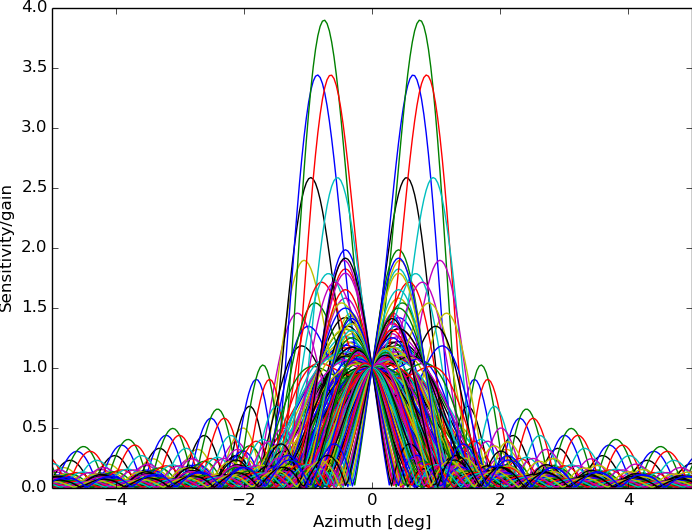
\includegraphics[width=0.49\linewidth]{gfx/1_window_response.png}}\hfill
\subfloat[Mean images]{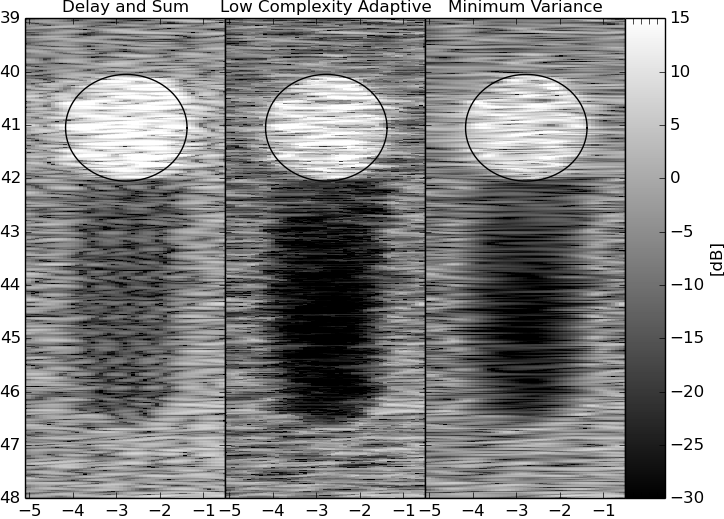
\includegraphics[width=0.49\linewidth]{gfx/1_mean_imgs.png}}\\
\subfloat[Windows ($\beta$)]{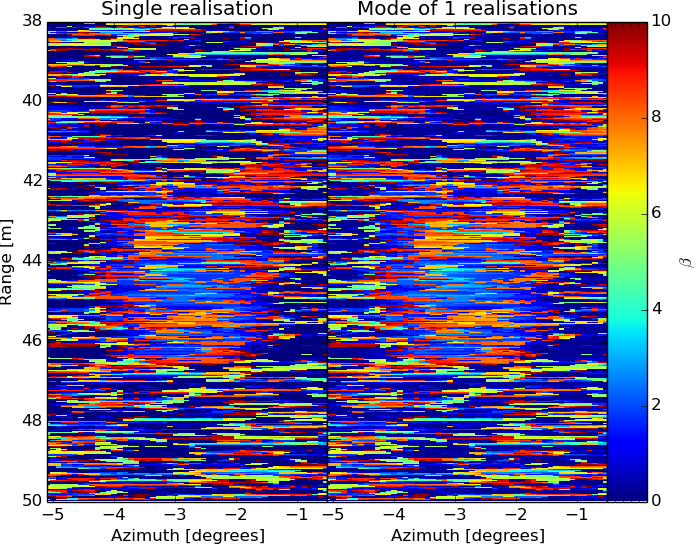
\includegraphics[width=0.49\linewidth]{gfx/1_windows_beta.png}}\hfill
\subfloat[Windows ($\phi$)]{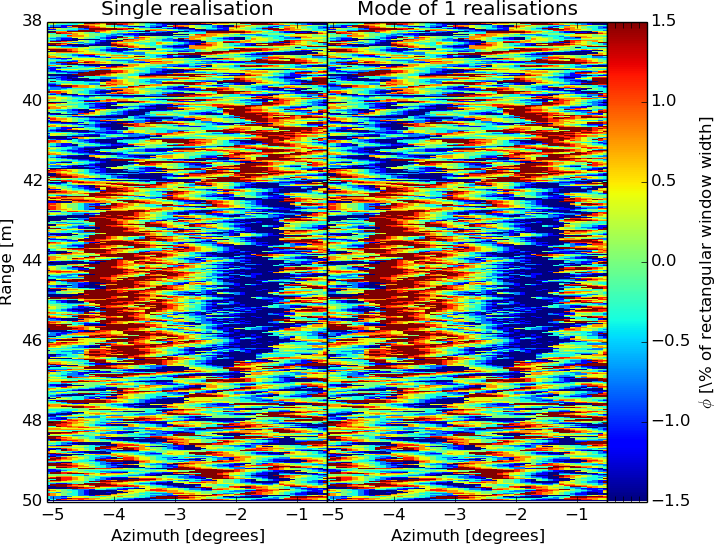
\includegraphics[width=0.48\linewidth]{gfx/1_windows_phi.png}}\\
\subfloat[Capon win. resp. through shadow]{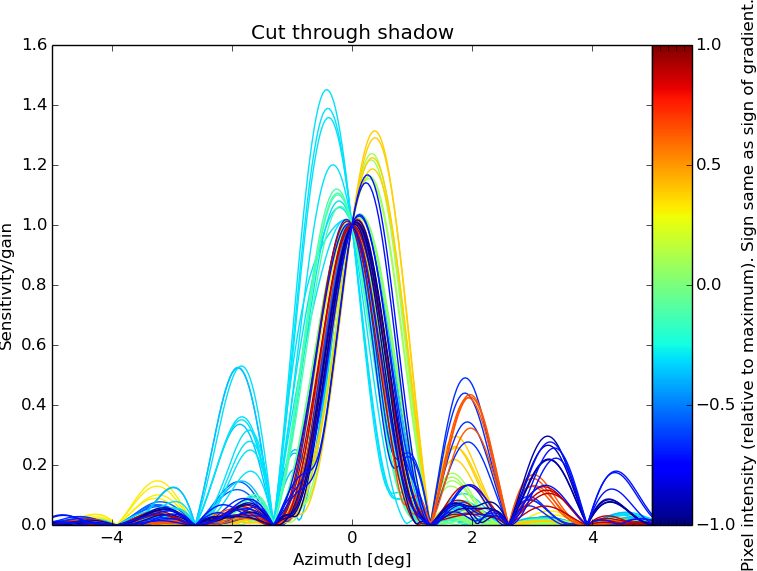
\includegraphics[width=0.49\linewidth]{gfx/1_win_resp_cut_shadow.png}}\hfill
\subfloat[Capon win. resp. through highlight]{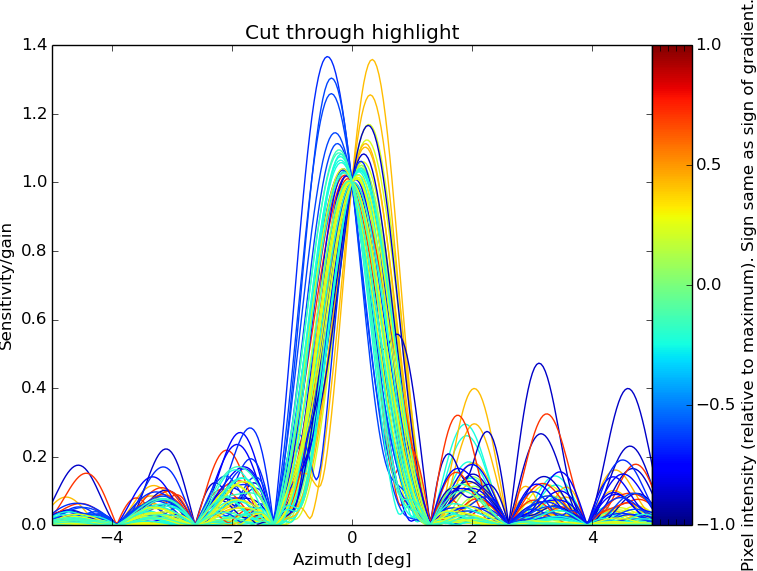
\includegraphics[width=0.49\linewidth]{gfx/1_win_resp_cut_highlight.png}}\\
\end{narrow}
\end{figure*}
\newpage
\begin{figure*}[!t]
\begin{narrow}{-1.2cm}{-1.2cm}\centering\vspace{-1.0cm}
\textbf{2. Capon: Tuning regularisation.}\\
\begin{tabular}[c]{l l l l}
\bf General & M = 32                            & $\Delta r = \frac{c}{2B}$ = 2.5 cm & $\frac{640\,\text{pixels}] / 12\,\text{m}}{\Delta r} = \frac{4}{3}$ \\
\bf LCA     & $\beta \in [0,10]$ (9 values) & $\phi \in [-1.07,1.07]$ deg (9 values) & Navg = 3 \\
\bf Capon   & $\Delta$ = 0.05                 & L = 16                           & Navg = 3 \\
\end{tabular}
\subfloat[LCA Window Response]{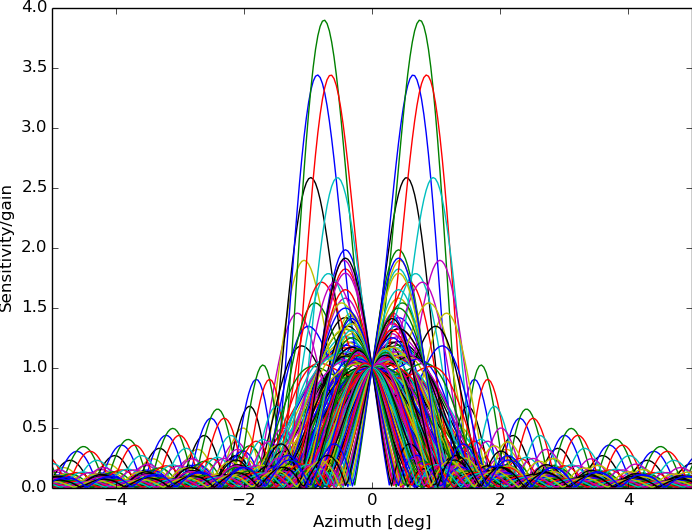
\includegraphics[width=0.49\linewidth]{gfx/2_window_response.png}}\hfill
\subfloat[Mean images]{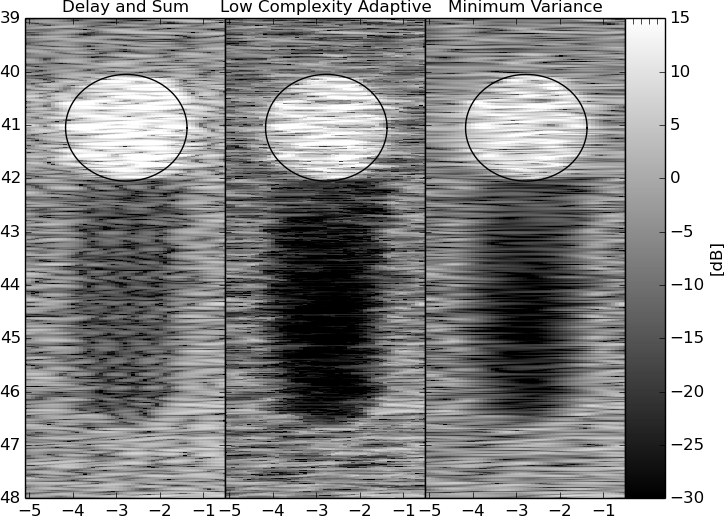
\includegraphics[width=0.49\linewidth]{gfx/2_mean_imgs.png}}\\
\subfloat[Windows ($\beta$)]{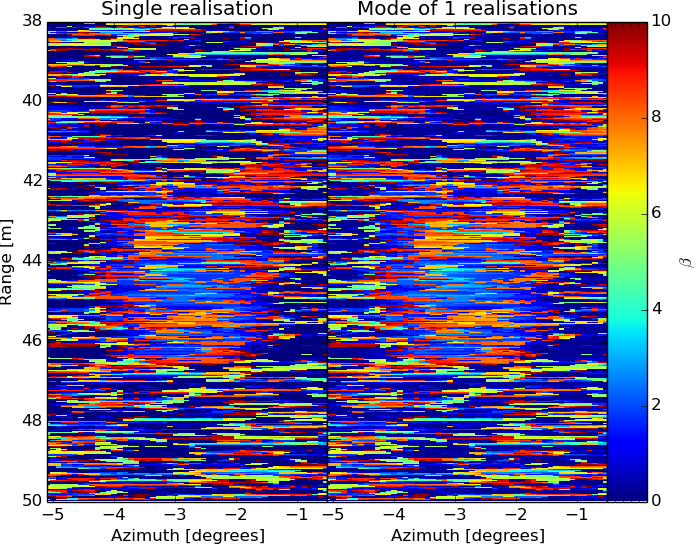
\includegraphics[width=0.49\linewidth]{gfx/2_windows_beta.png}}\hfill
\subfloat[Windows ($\phi$)]{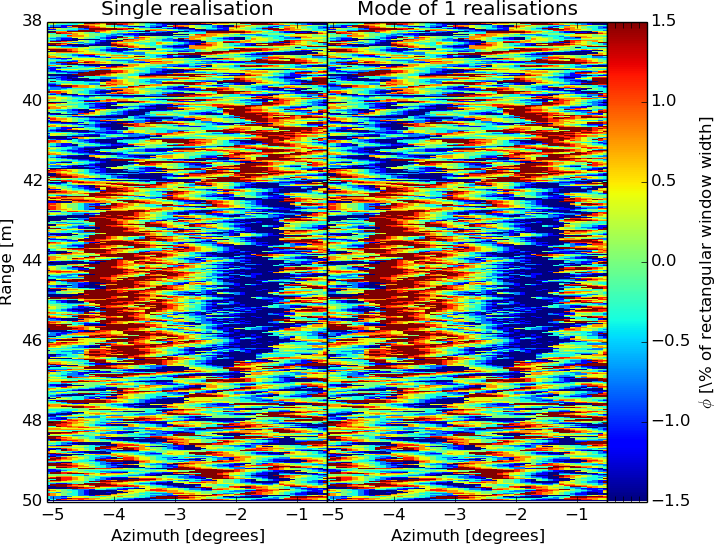
\includegraphics[width=0.48\linewidth]{gfx/2_windows_phi.png}}\\
\subfloat[Capon win. resp. through shadow]{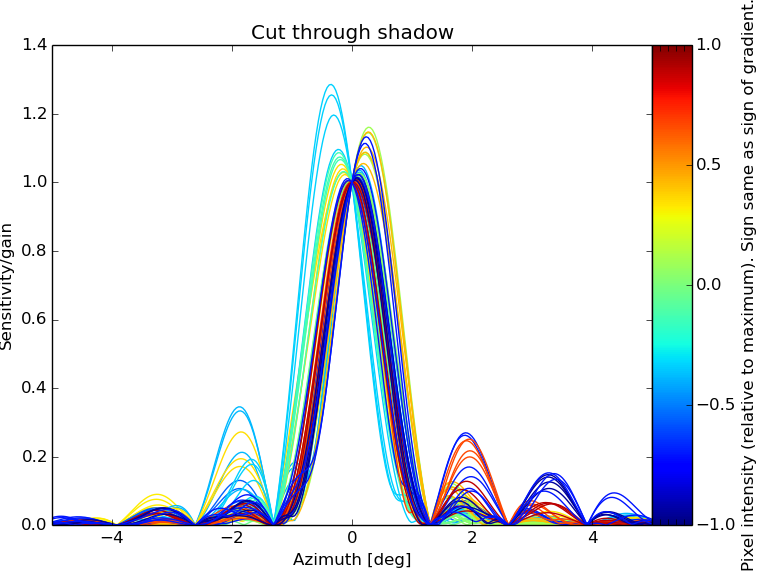
\includegraphics[width=0.49\linewidth]{gfx/2_win_resp_cut_shadow.png}}\hfill
\subfloat[Capon win. resp. through highlight]{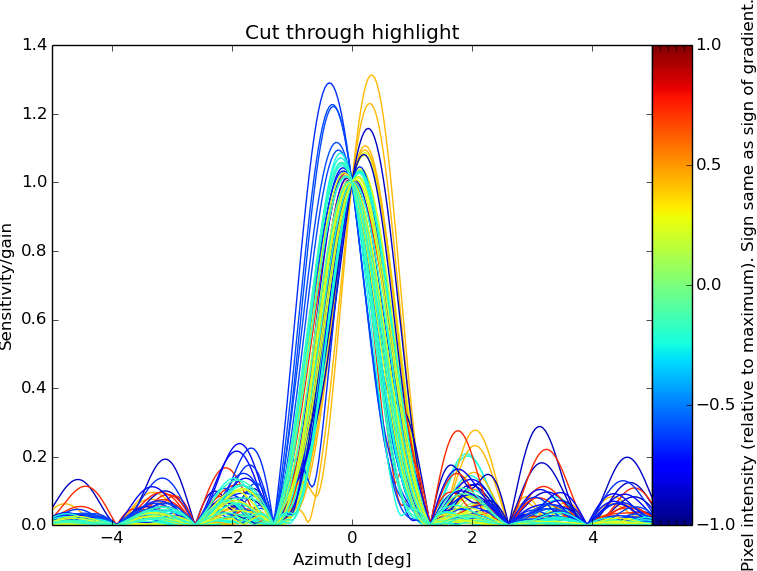
\includegraphics[width=0.49\linewidth]{gfx/2_win_resp_cut_highlight.png}}\\
\end{narrow}
\end{figure*}
\newpage
\begin{figure*}[!t]
\begin{narrow}{-1.2cm}{-1.2cm}\centering\vspace{-1.0cm}
\textbf{3. Capon: Tuning regularisation.}\\
\begin{tabular}[c]{l l l l}
\bf General & M = 32                            & $\Delta r = \frac{c}{2B}$ = 2.5 cm & $\frac{640\,\text{pixels}] / 12\,\text{m}}{\Delta r} = \frac{4}{3}$ \\
\bf LCA     & $\beta \in [0,10]$ (9 values) & $\phi \in [-1.07,1.07]$ deg (9 values) & Navg = 3 \\
\bf Capon   & $\Delta$ = 0.20                 & L = 16                           & Navg = 3 \\
\end{tabular}
\subfloat[LCA Window Response]{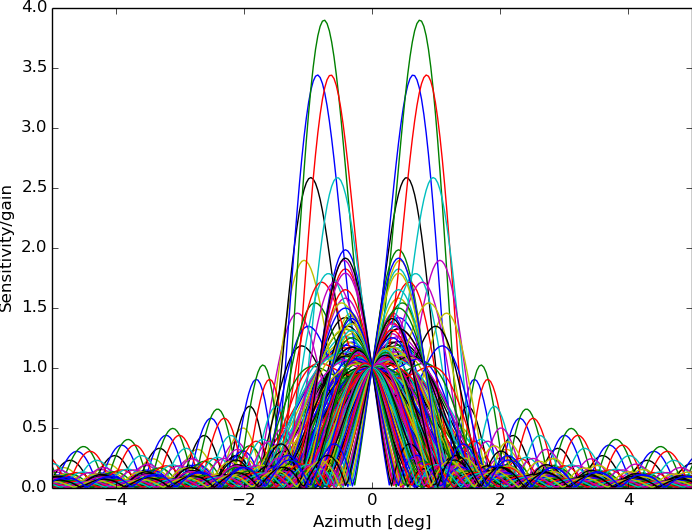
\includegraphics[width=0.49\linewidth]{gfx/3_window_response.png}}\hfill
\subfloat[Mean images]{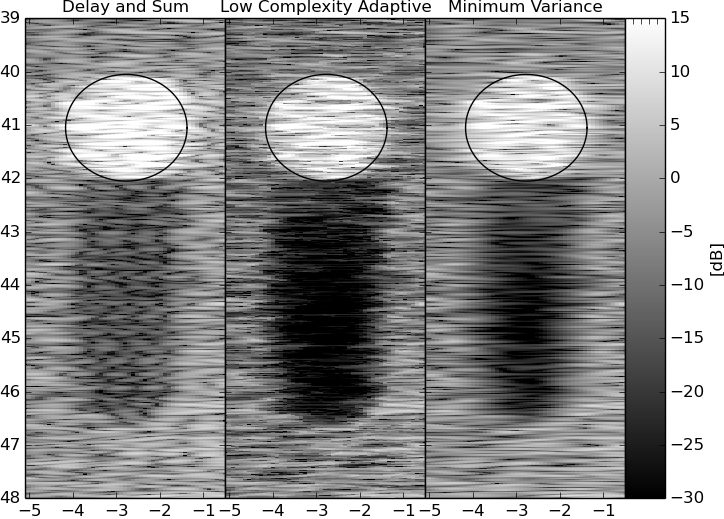
\includegraphics[width=0.49\linewidth]{gfx/3_mean_imgs.png}}\\
\subfloat[Windows ($\beta$)]{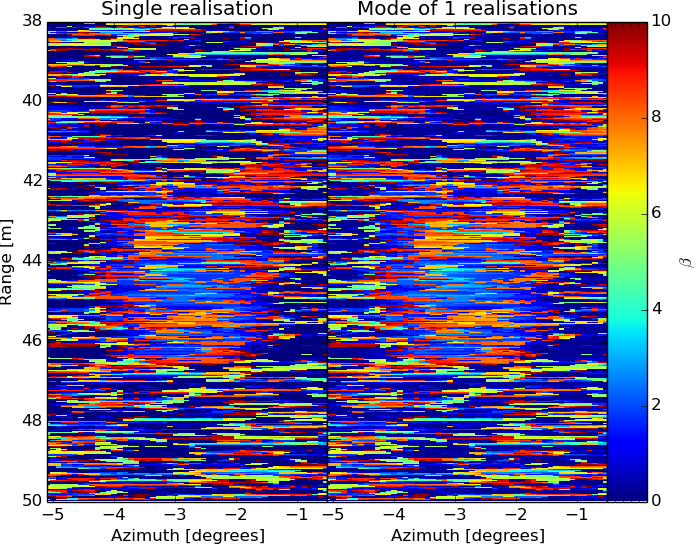
\includegraphics[width=0.49\linewidth]{gfx/3_windows_beta.png}}\hfill
\subfloat[Windows ($\phi$)]{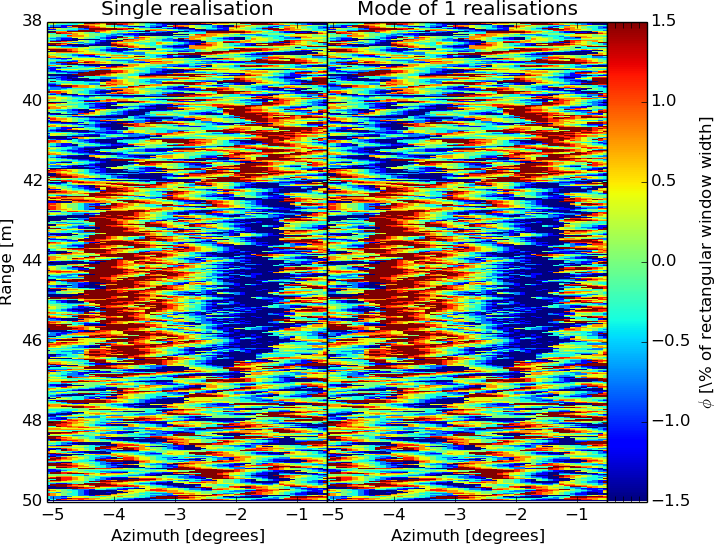
\includegraphics[width=0.48\linewidth]{gfx/3_windows_phi.png}}\\
\subfloat[Capon win. resp. through shadow]{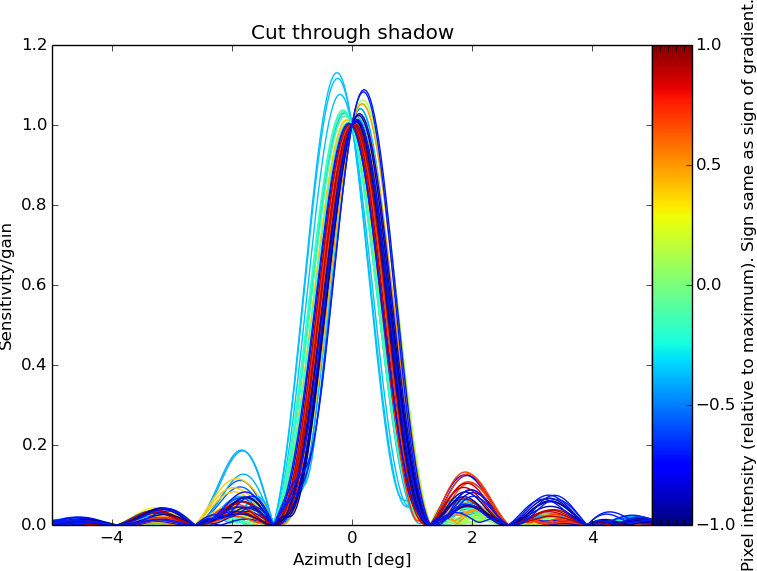
\includegraphics[width=0.49\linewidth]{gfx/3_win_resp_cut_shadow.png}}\hfill
\subfloat[Capon win. resp. through highlight]{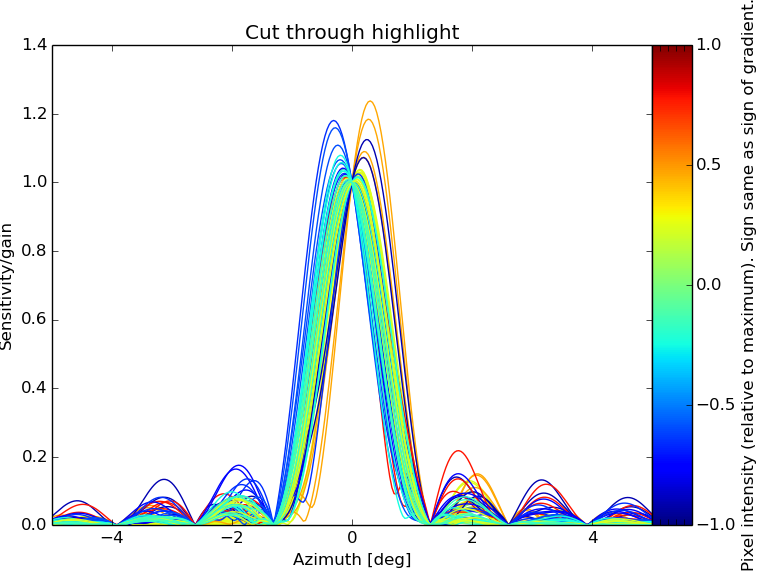
\includegraphics[width=0.49\linewidth]{gfx/3_win_resp_cut_highlight.png}}\\
\end{narrow}
\end{figure*}
\newpage
\begin{figure*}[!t]
\begin{narrow}{-1.2cm}{-1.2cm}\centering\vspace{-1.0cm}
\textbf{4. Capon: Tuning subarray.}\\
\begin{tabular}[c]{l l l l}
\bf General & M = 32                            & $\Delta r = \frac{c}{2B}$ = 2.5 cm & $\frac{640\,\text{pixels}] / 12\,\text{m}}{\Delta r} = \frac{4}{3}$ \\
\bf LCA     & $\beta \in [0,10]$ (9 values) & $\phi \in [-1.07,1.07]$ deg (9 values) & Navg = 3 \\
\bf Capon   & $\Delta$ = 0.01                 & L = 20                           & Navg = 3 \\
\end{tabular}
\subfloat[LCA Window Response]{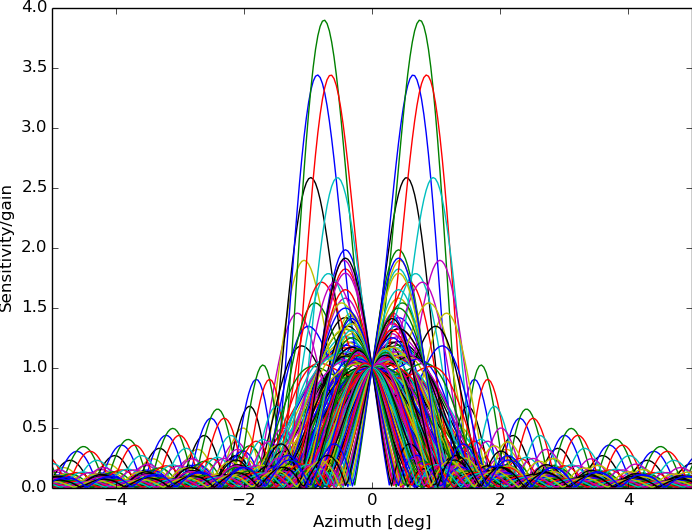
\includegraphics[width=0.49\linewidth]{gfx/4_window_response.png}}\hfill
\subfloat[Mean images]{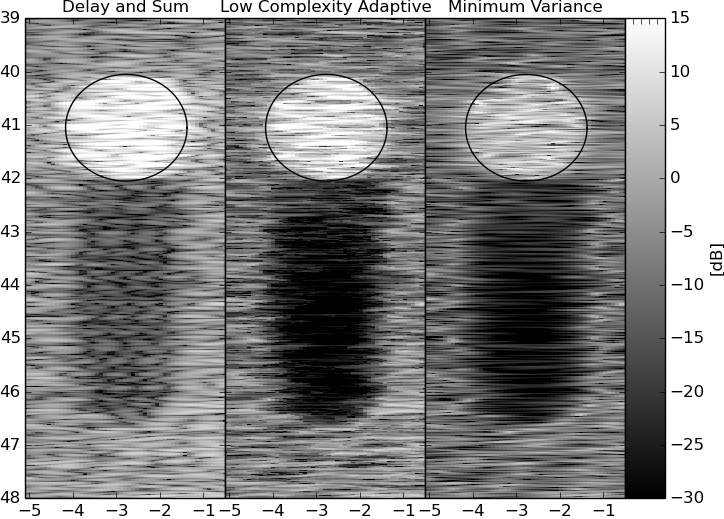
\includegraphics[width=0.49\linewidth]{gfx/4_mean_imgs.png}}\\
\subfloat[Windows ($\beta$)]{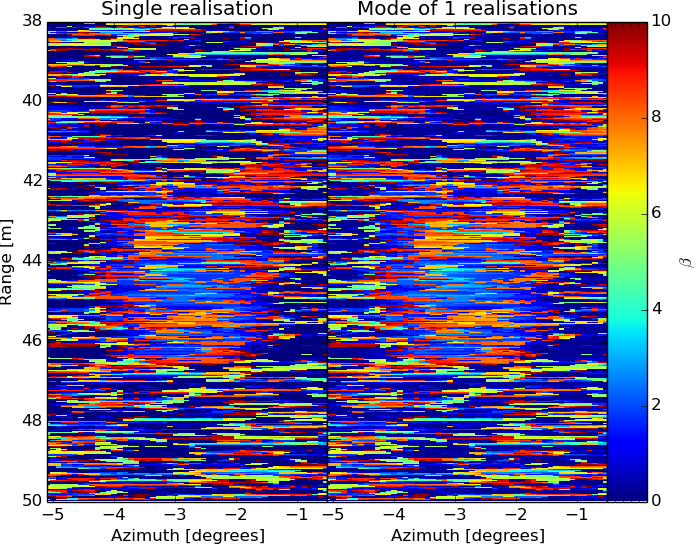
\includegraphics[width=0.49\linewidth]{gfx/4_windows_beta.png}}\hfill
\subfloat[Windows ($\phi$)]{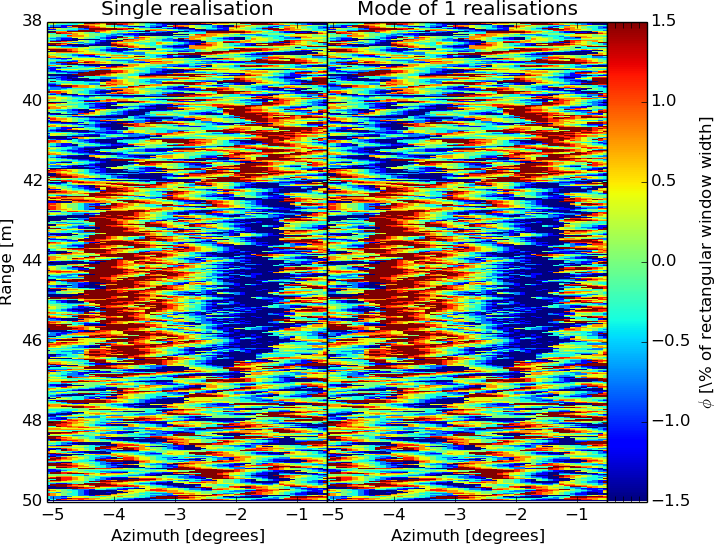
\includegraphics[width=0.48\linewidth]{gfx/4_windows_phi.png}}\\
\subfloat[Capon win. resp. through shadow]{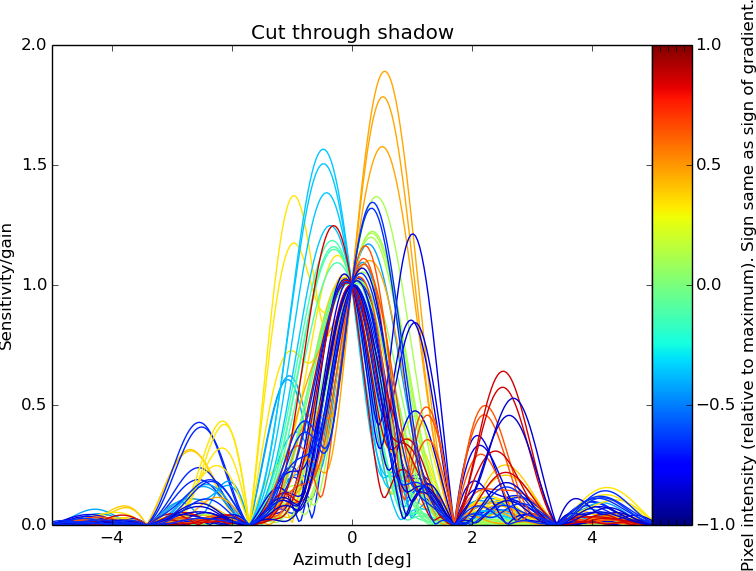
\includegraphics[width=0.49\linewidth]{gfx/4_win_resp_cut_shadow.png}}\hfill
\subfloat[Capon win. resp. through highlight]{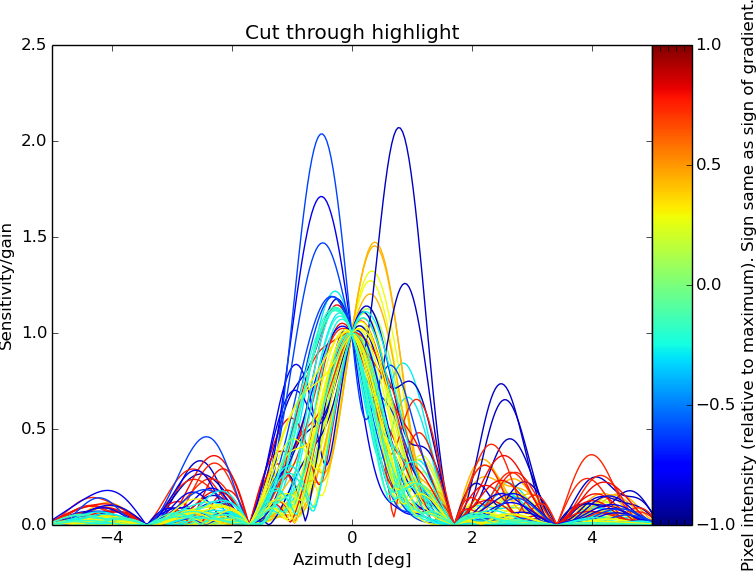
\includegraphics[width=0.49\linewidth]{gfx/4_win_resp_cut_highlight.png}}\\
\end{narrow}
\end{figure*}
\newpage
\begin{figure*}[!t]
\begin{narrow}{-1.2cm}{-1.2cm}\centering\vspace{-1.0cm}
\textbf{5. Capon: Tuning subarray.}\\
\begin{tabular}[c]{l l l l}
\bf General & M = 32                            & $\Delta r = \frac{c}{2B}$ = 2.5 cm & $\frac{640\,\text{pixels}] / 12\,\text{m}}{\Delta r} = \frac{4}{3}$ \\
\bf LCA     & $\beta \in [0,10]$ (9 values) & $\phi \in [-1.07,1.07]$ deg (9 values) & Navg = 3 \\
\bf Capon   & $\Delta$ = 0.01                 & L = 16                           & Navg = 3 \\
\end{tabular}
\subfloat[LCA Window Response]{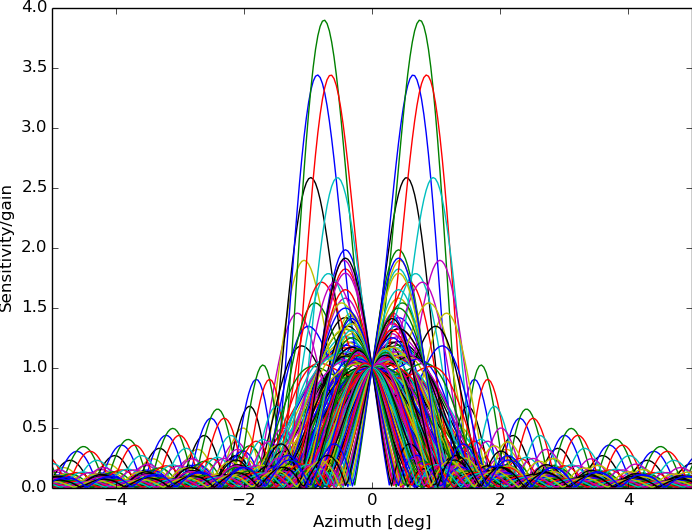
\includegraphics[width=0.49\linewidth]{gfx/5_window_response.png}}\hfill
\subfloat[Mean images]{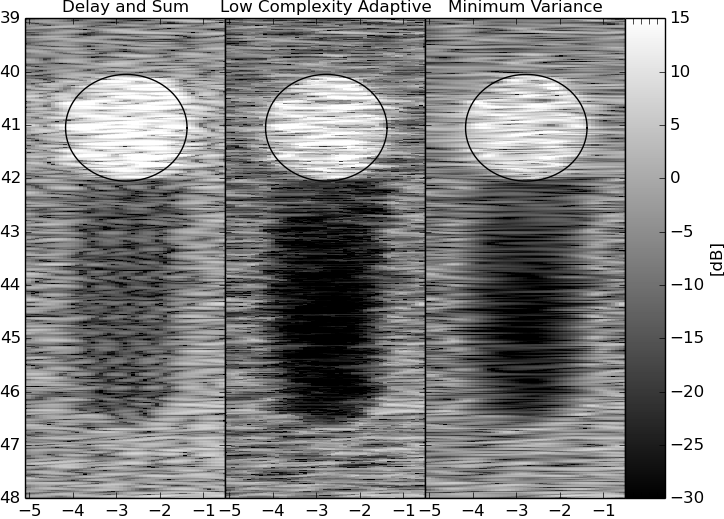
\includegraphics[width=0.49\linewidth]{gfx/5_mean_imgs.png}}\\
\subfloat[Windows ($\beta$)]{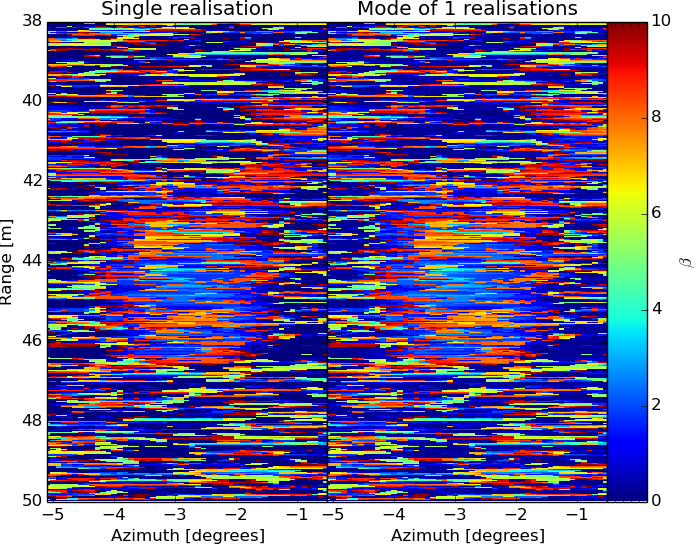
\includegraphics[width=0.49\linewidth]{gfx/5_windows_beta.png}}\hfill
\subfloat[Windows ($\phi$)]{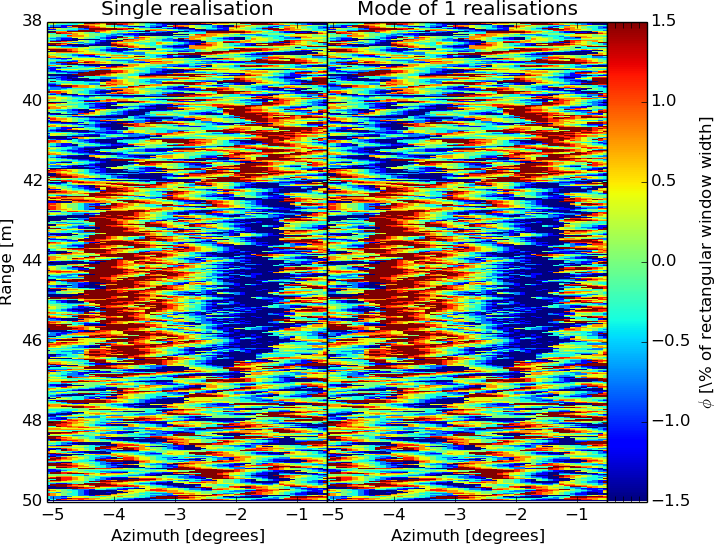
\includegraphics[width=0.48\linewidth]{gfx/5_windows_phi.png}}\\
\subfloat[Capon win. resp. through shadow]{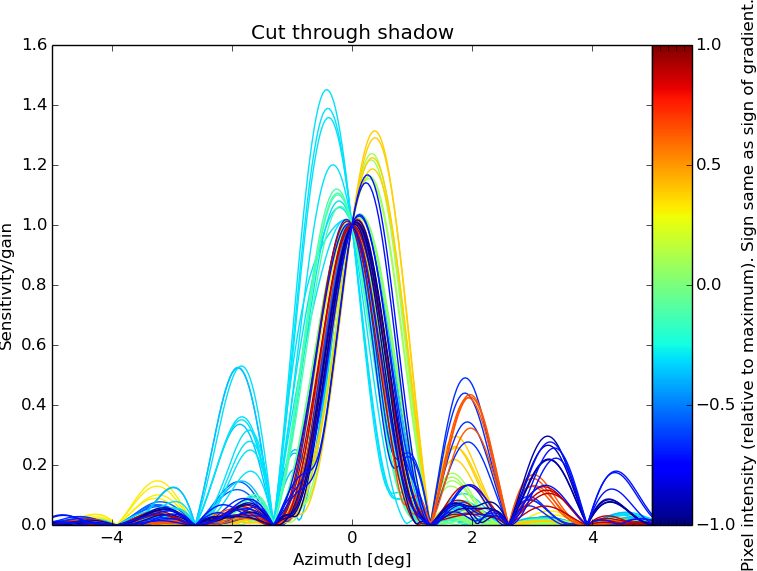
\includegraphics[width=0.49\linewidth]{gfx/5_win_resp_cut_shadow.png}}\hfill
\subfloat[Capon win. resp. through highlight]{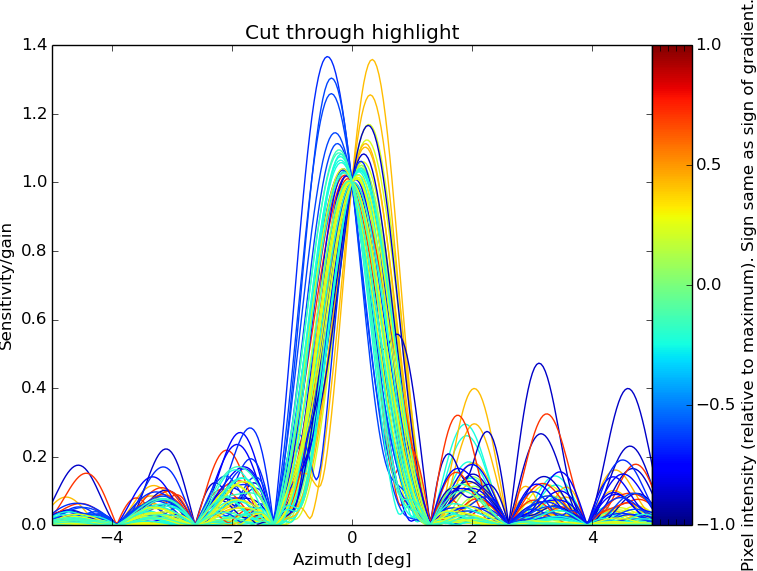
\includegraphics[width=0.49\linewidth]{gfx/5_win_resp_cut_highlight.png}}\\
\end{narrow}
\end{figure*}
\newpage
\begin{figure*}[!t]
\begin{narrow}{-1.2cm}{-1.2cm}\centering\vspace{-1.0cm}
\textbf{6. Capon: Tuning subarray.}\\
\begin{tabular}[c]{l l l l}
\bf General & M = 32                            & $\Delta r = \frac{c}{2B}$ = 2.5 cm & $\frac{640\,\text{pixels}] / 12\,\text{m}}{\Delta r} = \frac{4}{3}$ \\
\bf LCA     & $\beta \in [0,10]$ (9 values) & $\phi \in [-1.07,1.07]$ deg (9 values) & Navg = 3 \\
\bf Capon   & $\Delta$ = 0.01                 & L = 12                           & Navg = 3 \\
\end{tabular}
\subfloat[LCA Window Response]{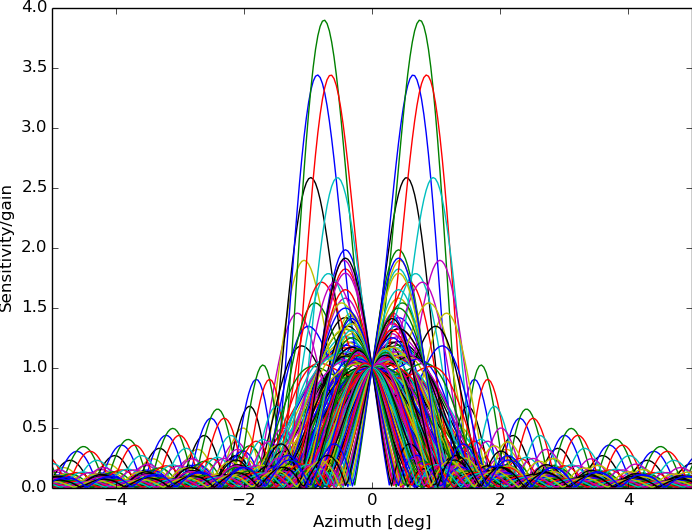
\includegraphics[width=0.49\linewidth]{gfx/6_window_response.png}}\hfill
\subfloat[Mean images]{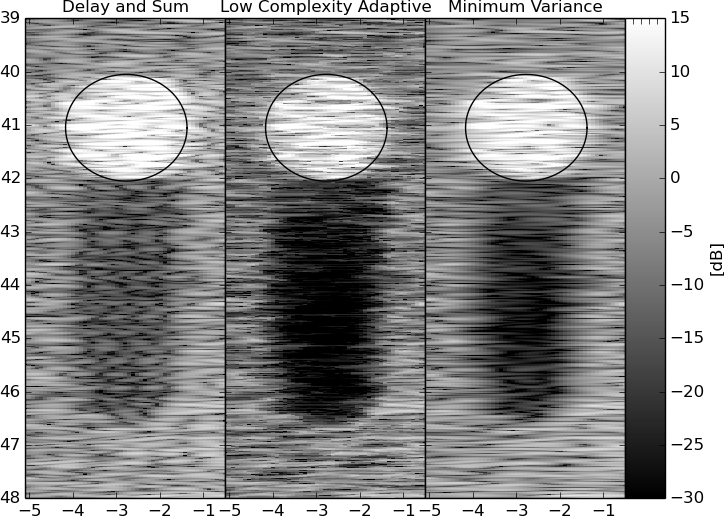
\includegraphics[width=0.49\linewidth]{gfx/6_mean_imgs.png}}\\
\subfloat[Windows ($\beta$)]{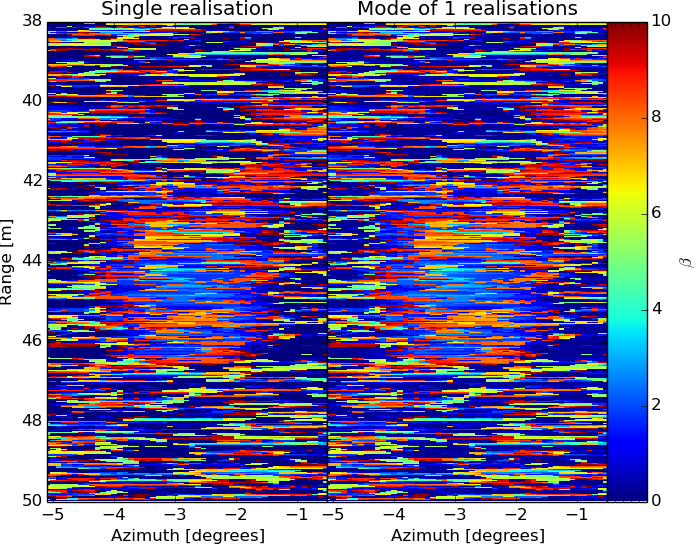
\includegraphics[width=0.49\linewidth]{gfx/6_windows_beta.png}}\hfill
\subfloat[Windows ($\phi$)]{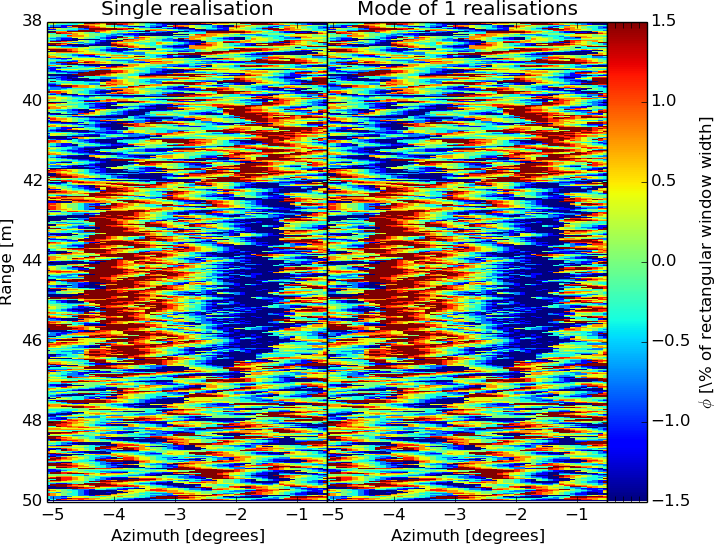
\includegraphics[width=0.48\linewidth]{gfx/6_windows_phi.png}}\\
\subfloat[Capon win. resp. through shadow]{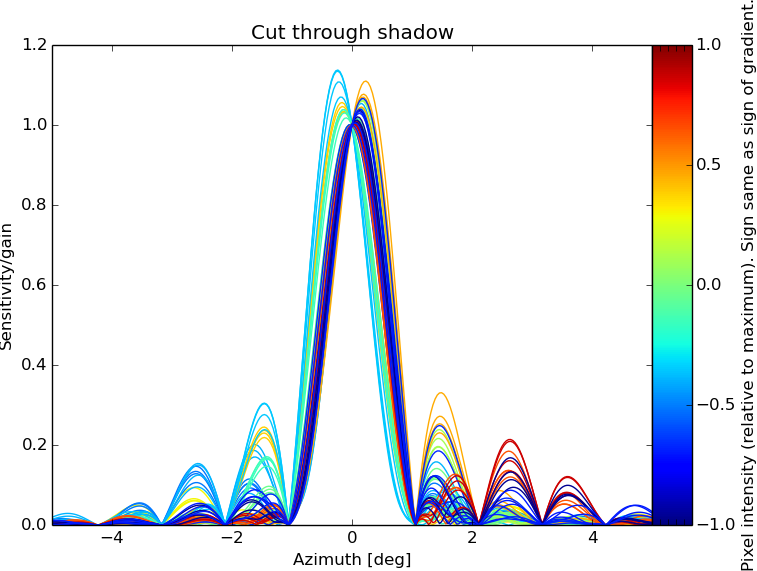
\includegraphics[width=0.49\linewidth]{gfx/6_win_resp_cut_shadow.png}}\hfill
\subfloat[Capon win. resp. through highlight]{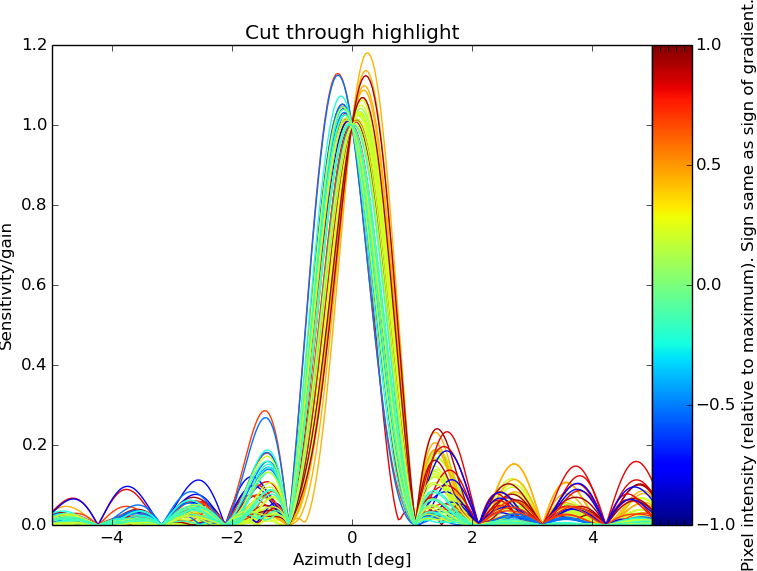
\includegraphics[width=0.49\linewidth]{gfx/6_win_resp_cut_highlight.png}}\\
\end{narrow}
\end{figure*}
\newpage
\begin{figure*}[!t]
\begin{narrow}{-1.2cm}{-1.2cm}\centering\vspace{-1.0cm}
\textbf{7. Capon: Tuning time averaging.}\\
\begin{tabular}[c]{l l l l}
\bf General & M = 32                            & $\Delta r = \frac{c}{2B}$ = 2.5 cm & $\frac{640\,\text{pixels}] / 12\,\text{m}}{\Delta r} = \frac{4}{3}$ \\
\bf LCA     & $\beta \in [0,10]$ (9 values) & $\phi \in [-1.07,1.07]$ deg (9 values) & Navg = 1 \\
\bf Capon   & $\Delta$ = 0.01                 & L = 16                           & Navg = 1 \\
\end{tabular}
\subfloat[LCA Window Response]{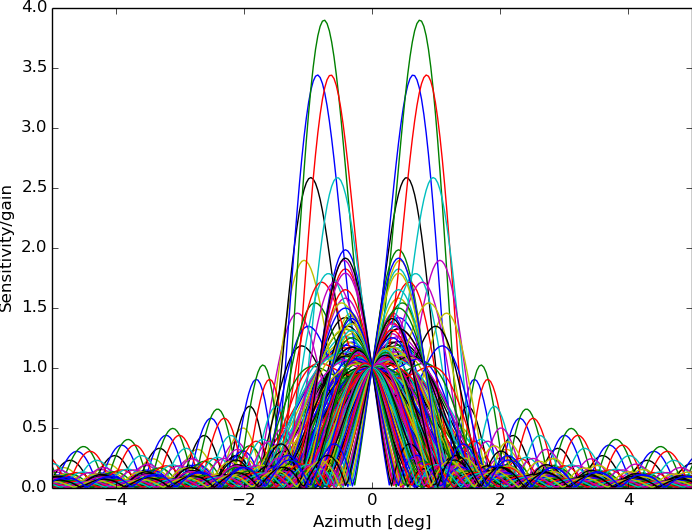
\includegraphics[width=0.49\linewidth]{gfx/7_window_response.png}}\hfill
\subfloat[Mean images]{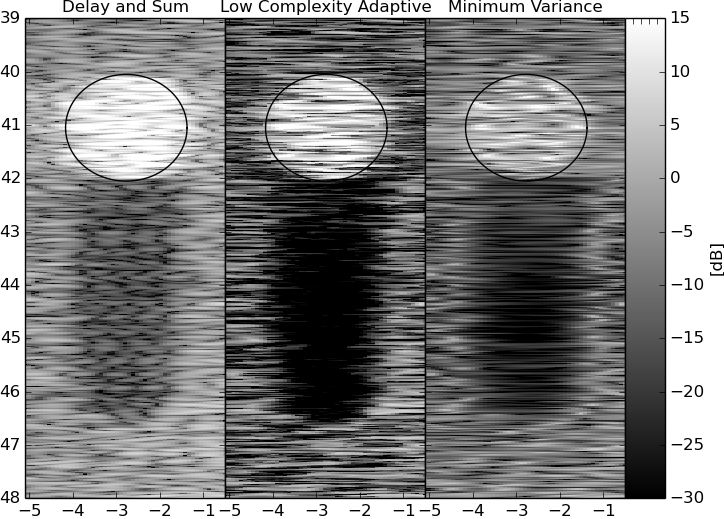
\includegraphics[width=0.49\linewidth]{gfx/7_mean_imgs.png}}\\
\subfloat[Windows ($\beta$)]{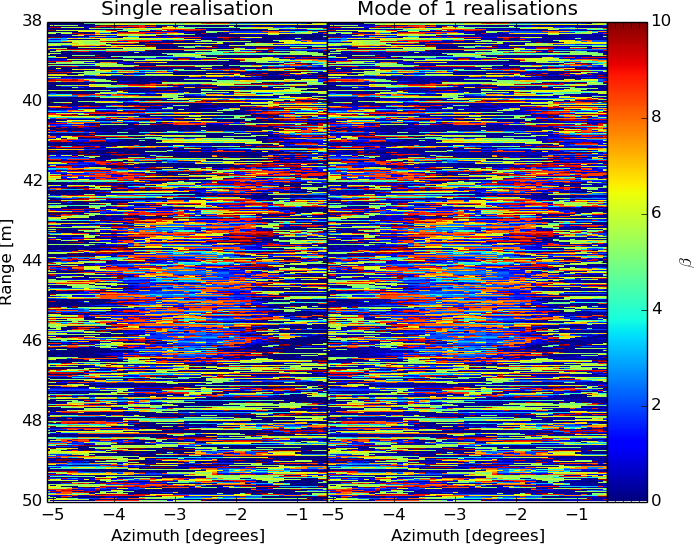
\includegraphics[width=0.49\linewidth]{gfx/7_windows_beta.png}}\hfill
\subfloat[Windows ($\phi$)]{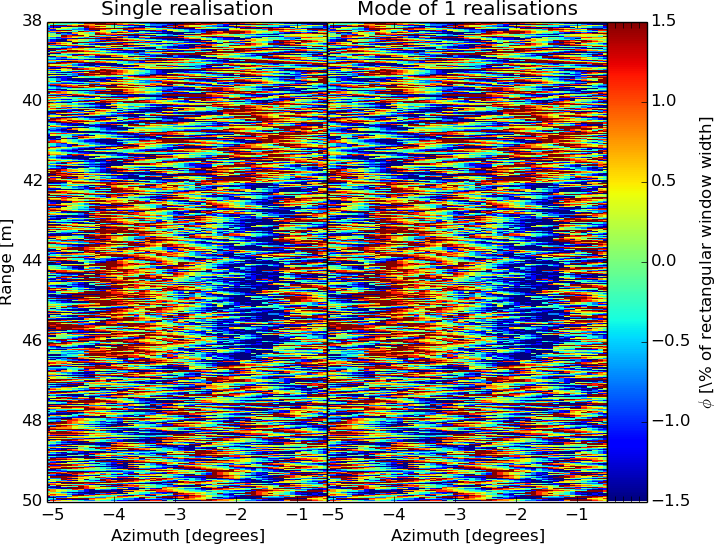
\includegraphics[width=0.48\linewidth]{gfx/7_windows_phi.png}}\\
\subfloat[Capon win. resp. through shadow]{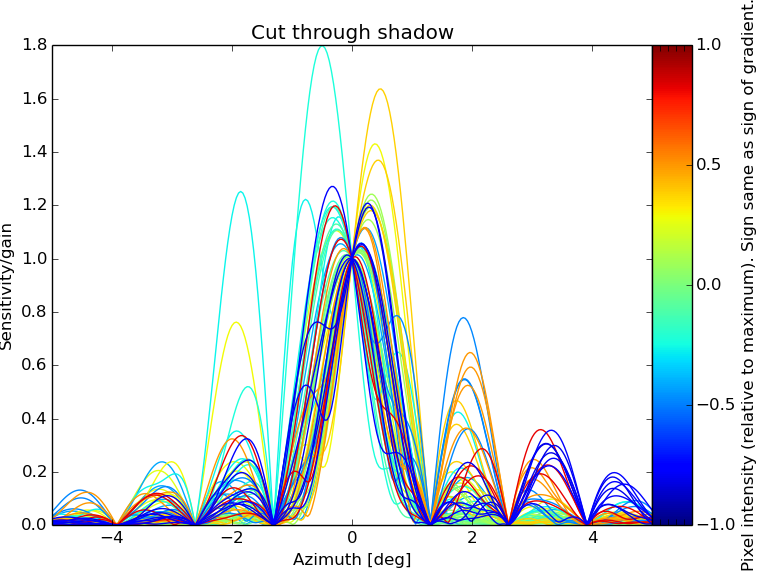
\includegraphics[width=0.49\linewidth]{gfx/7_win_resp_cut_shadow.png}}\hfill
\subfloat[Capon win. resp. through highlight]{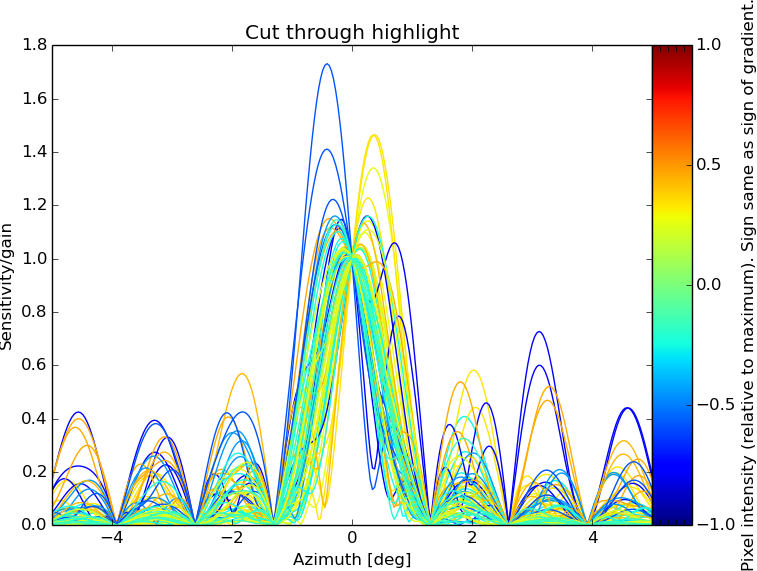
\includegraphics[width=0.49\linewidth]{gfx/7_win_resp_cut_highlight.png}}\\
\end{narrow}
\end{figure*}
\newpage
\begin{figure*}[!t]
\begin{narrow}{-1.2cm}{-1.2cm}\centering\vspace{-1.0cm}
\textbf{8. Capon: Tuning time averaging.}\\
\begin{tabular}[c]{l l l l}
\bf General & M = 32                            & $\Delta r = \frac{c}{2B}$ = 2.5 cm & $\frac{640\,\text{pixels}] / 12\,\text{m}}{\Delta r} = \frac{4}{3}$ \\
\bf LCA     & $\beta \in [0,10]$ (9 values) & $\phi \in [-1.07,1.07]$ deg (9 values) & Navg = 3 \\
\bf Capon   & $\Delta$ = 0.01                 & L = 16                           & Navg = 3 \\
\end{tabular}
\subfloat[LCA Window Response]{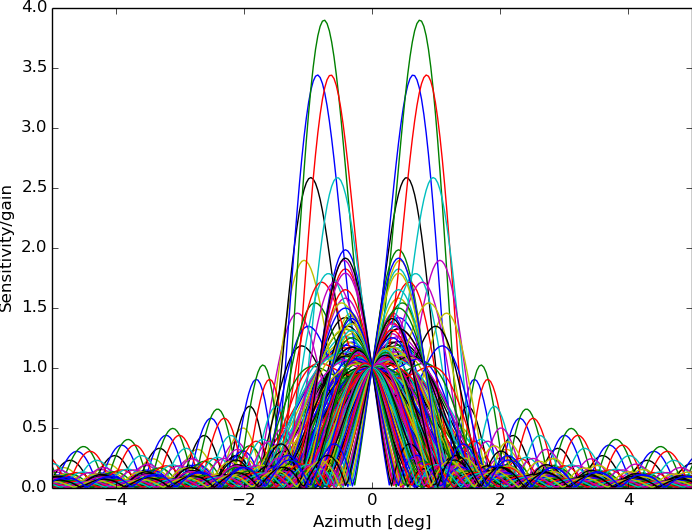
\includegraphics[width=0.49\linewidth]{gfx/8_window_response.png}}\hfill
\subfloat[Mean images]{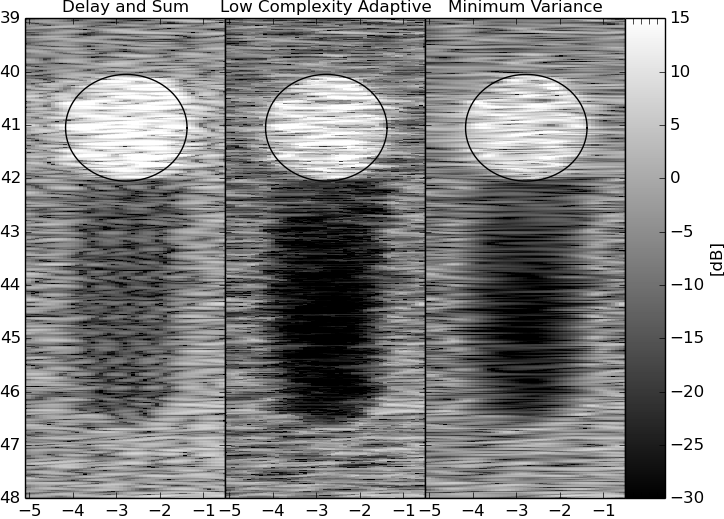
\includegraphics[width=0.49\linewidth]{gfx/8_mean_imgs.png}}\\
\subfloat[Windows ($\beta$)]{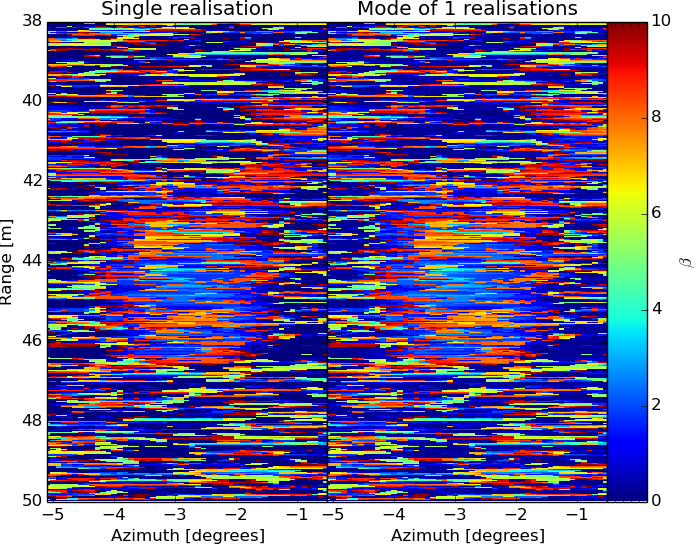
\includegraphics[width=0.49\linewidth]{gfx/8_windows_beta.png}}\hfill
\subfloat[Windows ($\phi$)]{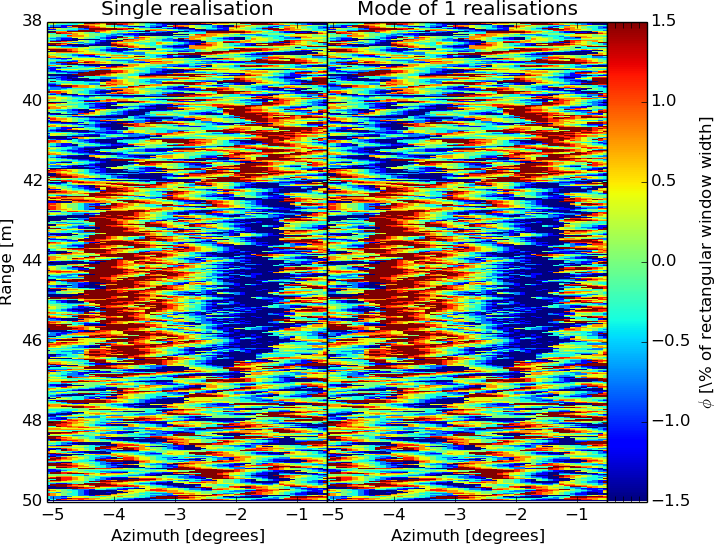
\includegraphics[width=0.48\linewidth]{gfx/8_windows_phi.png}}\\
\subfloat[Capon win. resp. through shadow]{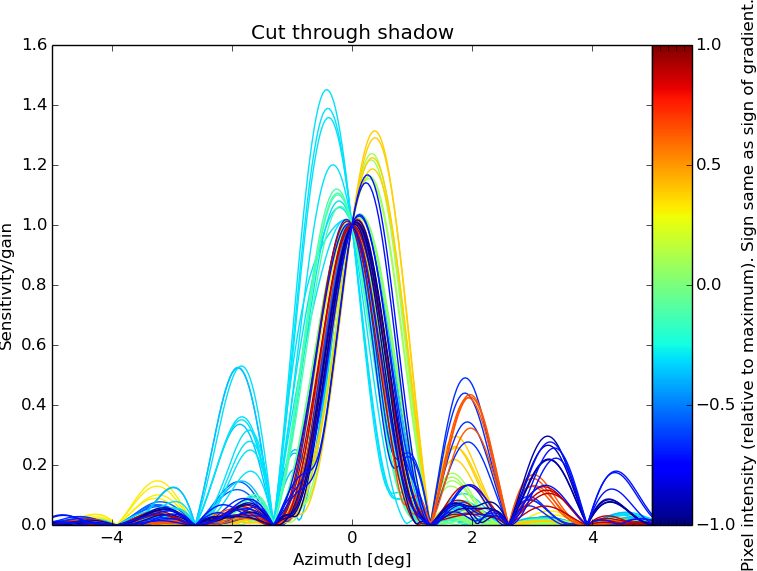
\includegraphics[width=0.49\linewidth]{gfx/8_win_resp_cut_shadow.png}}\hfill
\subfloat[Capon win. resp. through highlight]{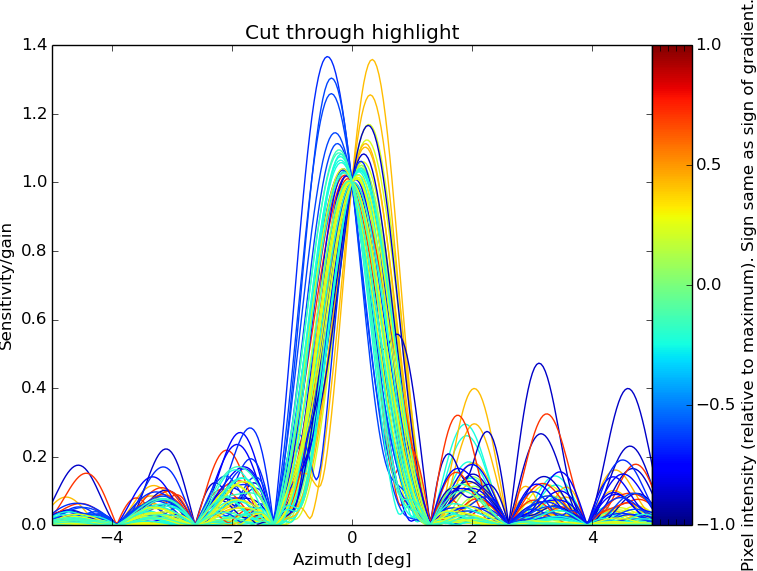
\includegraphics[width=0.49\linewidth]{gfx/8_win_resp_cut_highlight.png}}\\
\end{narrow}
\end{figure*}
\newpage
\begin{figure*}[!t]
\begin{narrow}{-1.2cm}{-1.2cm}\centering\vspace{-1.0cm}
\textbf{9. Capon: Tuning time averaging.}\\
\begin{tabular}[c]{l l l l}
\bf General & M = 32                            & $\Delta r = \frac{c}{2B}$ = 2.5 cm & $\frac{640\,\text{pixels}] / 12\,\text{m}}{\Delta r} = \frac{4}{3}$ \\
\bf LCA     & $\beta \in [0,10]$ (9 values) & $\phi \in [-1.07,1.07]$ deg (9 values) & Navg = 5 \\
\bf Capon   & $\Delta$ = 0.01                 & L = 16                           & Navg = 5 \\
\end{tabular}
\subfloat[LCA Window Response]{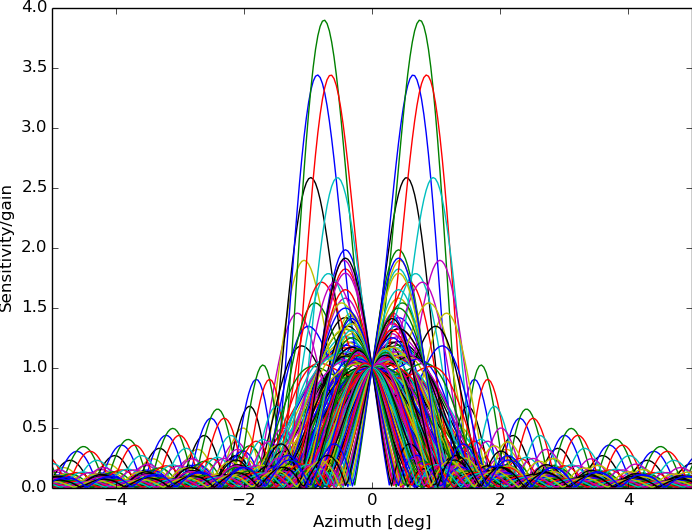
\includegraphics[width=0.49\linewidth]{gfx/9_window_response.png}}\hfill
\subfloat[Mean images]{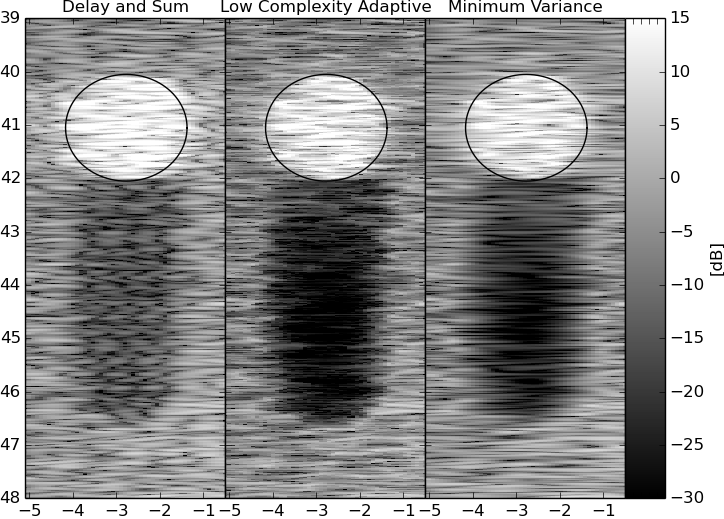
\includegraphics[width=0.49\linewidth]{gfx/9_mean_imgs.png}}\\
\subfloat[Windows ($\beta$)]{\includegraphics[width=0.49\linewidth]{gfx/9_windows_beta.png}}\hfill
\subfloat[Windows ($\phi$)]{\includegraphics[width=0.48\linewidth]{gfx/9_windows_phi.png}}\\
\subfloat[Capon win. resp. through shadow]{\includegraphics[width=0.49\linewidth]{gfx/9_win_resp_cut_shadow.png}}\hfill
\subfloat[Capon win. resp. through highlight]{\includegraphics[width=0.49\linewidth]{gfx/9_win_resp_cut_highlight.png}}\\
\end{narrow}
\end{figure*}
\newpage
\begin{figure*}[!t]
\begin{narrow}{-1.2cm}{-1.2cm}\centering\vspace{-1.0cm}
\textbf{10. Capon: Tuning time averaging.}\\
\begin{tabular}[c]{l l l l}
\bf General & M = 32                            & $\Delta r = \frac{c}{2B}$ = 2.5 cm & $\frac{640\,\text{pixels}] / 12\,\text{m}}{\Delta r} = \frac{4}{3}$ \\
\bf LCA     & $\beta \in [0,10]$ (9 values) & $\phi \in [-1.07,1.07]$ deg (9 values) & Navg = 7 \\
\bf Capon   & $\Delta$ = 0.01                 & L = 16                           & Navg = 7 \\
\end{tabular}
\subfloat[LCA Window Response]{\includegraphics[width=0.49\linewidth]{gfx/10_window_response.png}}\hfill
\subfloat[Mean images]{\includegraphics[width=0.49\linewidth]{gfx/10_mean_imgs.png}}\\
\subfloat[Windows ($\beta$)]{\includegraphics[width=0.49\linewidth]{gfx/10_windows_beta.png}}\hfill
\subfloat[Windows ($\phi$)]{\includegraphics[width=0.48\linewidth]{gfx/10_windows_phi.png}}\\
\subfloat[Capon win. resp. through shadow]{\includegraphics[width=0.49\linewidth]{gfx/10_win_resp_cut_shadow.png}}\hfill
\subfloat[Capon win. resp. through highlight]{\includegraphics[width=0.49\linewidth]{gfx/10_win_resp_cut_highlight.png}}\\
\end{narrow}
\end{figure*}
\newpage
\begin{figure*}[!t]
\begin{narrow}{-1.2cm}{-1.2cm}\centering\vspace{-1.0cm}
\textbf{11. LCA: Reasonable settings.}\\
\begin{tabular}[c]{l l l l}
\bf General & M = 32                            & $\Delta r = \frac{c}{2B}$ = 2.5 cm & $\frac{640\,\text{pixels}] / 12\,\text{m}}{\Delta r} = \frac{4}{3}$ \\
\bf LCA     & $\beta \in [0,10]$ (9 values) & $\phi \in [-0.57,0.57]$ deg (9 values) & Navg = 7 \\
\bf Capon   & $\Delta$ = 0.01                 & L = 16                           & Navg = 7 \\
\end{tabular}
\subfloat[LCA Window Response]{\includegraphics[width=0.49\linewidth]{gfx/11_window_response.png}}\hfill
\subfloat[Mean images]{\includegraphics[width=0.49\linewidth]{gfx/11_mean_imgs.png}}\\
\subfloat[Windows ($\beta$)]{\includegraphics[width=0.49\linewidth]{gfx/11_windows_beta.png}}\hfill
\subfloat[Windows ($\phi$)]{\includegraphics[width=0.48\linewidth]{gfx/11_windows_phi.png}}\\
\subfloat[Capon win. resp. through shadow]{\includegraphics[width=0.49\linewidth]{gfx/11_win_resp_cut_shadow.png}}\hfill
\subfloat[Capon win. resp. through highlight]{\includegraphics[width=0.49\linewidth]{gfx/11_win_resp_cut_highlight.png}}\\
\end{narrow}
\end{figure*}
\newpage
\begin{figure*}[!t]
\begin{narrow}{-1.2cm}{-1.2cm}\centering\vspace{-1.0cm}
\textbf{12. LCA: Lots of Kaiser windows - wide span.}\\
\begin{tabular}[c]{l l l l}
\bf General & M = 32                            & $\Delta r = \frac{c}{2B}$ = 2.5 cm & $\frac{640\,\text{pixels}] / 12\,\text{m}}{\Delta r} = \frac{4}{3}$ \\
\bf LCA     & $\beta \in [0,20]$ (19 values) & $\phi \in [-1.07,1.07]$ deg (19 values) & Navg = 7 \\
\bf Capon   & $\Delta$ = 0.01                 & L = 16                           & Navg = 7 \\
\end{tabular}
\subfloat[LCA Window Response]{\includegraphics[width=0.49\linewidth]{gfx/12_window_response.png}}\hfill
\subfloat[Mean images]{\includegraphics[width=0.49\linewidth]{gfx/12_mean_imgs.png}}\\
\subfloat[Windows ($\beta$)]{\includegraphics[width=0.49\linewidth]{gfx/12_windows_beta.png}}\hfill
\subfloat[Windows ($\phi$)]{\includegraphics[width=0.48\linewidth]{gfx/12_windows_phi.png}}\\
\subfloat[Capon win. resp. through shadow]{\includegraphics[width=0.49\linewidth]{gfx/12_win_resp_cut_shadow.png}}\hfill
\subfloat[Capon win. resp. through highlight]{\includegraphics[width=0.49\linewidth]{gfx/12_win_resp_cut_highlight.png}}\\
\end{narrow}
\end{figure*}
\newpage
\begin{figure*}[!t]
\begin{narrow}{-1.2cm}{-1.2cm}\centering\vspace{-1.0cm}
\textbf{13. LCA: Lots of trigonometric windows - wide span.}\\
\begin{tabular}[c]{l l l l}
\bf General & M = 32                            & $\Delta r = \frac{c}{2B}$ = 2.5 cm & $\frac{640\,\text{pixels}] / 12\,\text{m}}{\Delta r} = \frac{4}{3}$ \\
\bf LCA     & $\beta \in [0,20]$ (19 values) & $\phi \in [-1.07,1.07]$ deg (19 values) & Navg = 7 \\
\bf Capon   & $\Delta$ = 0.01                 & L = 16                           & Navg = 7 \\
\end{tabular}
\subfloat[LCA Window Response]{\includegraphics[width=0.49\linewidth]{gfx/13_window_response.png}}\hfill
\subfloat[Mean images]{\includegraphics[width=0.49\linewidth]{gfx/13_mean_imgs.png}}\\
\subfloat[Windows ($\beta$)]{\includegraphics[width=0.49\linewidth]{gfx/13_windows_beta.png}}\hfill
\subfloat[Windows ($\phi$)]{\includegraphics[width=0.48\linewidth]{gfx/13_windows_phi.png}}\\
\subfloat[Capon win. resp. through shadow]{\includegraphics[width=0.49\linewidth]{gfx/13_win_resp_cut_shadow.png}}\hfill
\subfloat[Capon win. resp. through highlight]{\includegraphics[width=0.49\linewidth]{gfx/13_win_resp_cut_highlight.png}}\\
\end{narrow}
\end{figure*}
\newpage
\begin{figure*}[!t]
\begin{narrow}{-1.2cm}{-1.2cm}\centering\vspace{-1.0cm}
\textbf{14. LCA: Back on Kaiser - reducing steering span.}\\
\begin{tabular}[c]{l l l l}
\bf General & M = 32                            & $\Delta r = \frac{c}{2B}$ = 2.5 cm & $\frac{640\,\text{pixels}] / 12\,\text{m}}{\Delta r} = \frac{4}{3}$ \\
\bf LCA     & $\beta \in [0,20]$ (19 values) & $\phi \in [-0.72,0.72]$ deg (19 values) & Navg = 7 \\
\bf Capon   & $\Delta$ = 0.01                 & L = 16                           & Navg = 7 \\
\end{tabular}
\subfloat[LCA Window Response]{\includegraphics[width=0.49\linewidth]{gfx/14_window_response.png}}\hfill
\subfloat[Mean images]{\includegraphics[width=0.49\linewidth]{gfx/14_mean_imgs.png}}\\
\subfloat[Windows ($\beta$)]{\includegraphics[width=0.49\linewidth]{gfx/14_windows_beta.png}}\hfill
\subfloat[Windows ($\phi$)]{\includegraphics[width=0.48\linewidth]{gfx/14_windows_phi.png}}\\
\subfloat[Capon win. resp. through shadow]{\includegraphics[width=0.49\linewidth]{gfx/14_win_resp_cut_shadow.png}}\hfill
\subfloat[Capon win. resp. through highlight]{\includegraphics[width=0.49\linewidth]{gfx/14_win_resp_cut_highlight.png}}\\
\end{narrow}
\end{figure*}
\newpage
\begin{figure*}[!t]
\begin{narrow}{-1.2cm}{-1.2cm}\centering\vspace{-1.0cm}
\textbf{15. LCA: Reducing steering span.}\\
\begin{tabular}[c]{l l l l}
\bf General & M = 32                            & $\Delta r = \frac{c}{2B}$ = 2.5 cm & $\frac{640\,\text{pixels}] / 12\,\text{m}}{\Delta r} = \frac{4}{3}$ \\
\bf LCA     & $\beta \in [0,20]$ (19 values) & $\phi \in [-0.36,0.36]$ deg (19 values) & Navg = 7 \\
\bf Capon   & $\Delta$ = 0.01                 & L = 16                           & Navg = 7 \\
\end{tabular}
\subfloat[LCA Window Response]{\includegraphics[width=0.49\linewidth]{gfx/15_window_response.png}}\hfill
\subfloat[Mean images]{\includegraphics[width=0.49\linewidth]{gfx/15_mean_imgs.png}}\\
\subfloat[Windows ($\beta$)]{\includegraphics[width=0.49\linewidth]{gfx/15_windows_beta.png}}\hfill
\subfloat[Windows ($\phi$)]{\includegraphics[width=0.48\linewidth]{gfx/15_windows_phi.png}}\\
\subfloat[Capon win. resp. through shadow]{\includegraphics[width=0.49\linewidth]{gfx/15_win_resp_cut_shadow.png}}\hfill
\subfloat[Capon win. resp. through highlight]{\includegraphics[width=0.49\linewidth]{gfx/15_win_resp_cut_highlight.png}}\\
\end{narrow}
\end{figure*}
\newpage
\begin{figure*}[!t]
\begin{narrow}{-1.2cm}{-1.2cm}\centering\vspace{-1.0cm}
\textbf{16. LCA: Adjusting resolution/SNR.}\\
\begin{tabular}[c]{l l l l}
\bf General & M = 32                            & $\Delta r = \frac{c}{2B}$ = 2.5 cm & $\frac{640\,\text{pixels}] / 12\,\text{m}}{\Delta r} = \frac{4}{3}$ \\
\bf LCA     & $\beta \in [0,5]$ (19 values) & $\phi \in [-0.72,0.72]$ deg (19 values) & Navg = 7 \\
\bf Capon   & $\Delta$ = 0.01                 & L = 16                           & Navg = 7 \\
\end{tabular}
\subfloat[LCA Window Response]{\includegraphics[width=0.49\linewidth]{gfx/16_window_response.png}}\hfill
\subfloat[Mean images]{\includegraphics[width=0.49\linewidth]{gfx/16_mean_imgs.png}}\\
\subfloat[Windows ($\beta$)]{\includegraphics[width=0.49\linewidth]{gfx/16_windows_beta.png}}\hfill
\subfloat[Windows ($\phi$)]{\includegraphics[width=0.48\linewidth]{gfx/16_windows_phi.png}}\\
\subfloat[Capon win. resp. through shadow]{\includegraphics[width=0.49\linewidth]{gfx/16_win_resp_cut_shadow.png}}\hfill
\subfloat[Capon win. resp. through highlight]{\includegraphics[width=0.49\linewidth]{gfx/16_win_resp_cut_highlight.png}}\\
\end{narrow}
\end{figure*}
\newpage
\begin{figure*}[!t]
\begin{narrow}{-1.2cm}{-1.2cm}\centering\vspace{-1.0cm}
\textbf{17. LCA: Adjusting resolution/SNR.}\\
\begin{tabular}[c]{l l l l}
\bf General & M = 32                            & $\Delta r = \frac{c}{2B}$ = 2.5 cm & $\frac{640\,\text{pixels}] / 12\,\text{m}}{\Delta r} = \frac{4}{3}$ \\
\bf LCA     & $\beta \in [5,20]$ (19 values) & $\phi \in [-0.72,0.72]$ deg (19 values) & Navg = 7 \\
\bf Capon   & $\Delta$ = 0.01                 & L = 16                           & Navg = 7 \\
\end{tabular}
\subfloat[LCA Window Response]{\includegraphics[width=0.49\linewidth]{gfx/17_window_response.png}}\hfill
\subfloat[Mean images]{\includegraphics[width=0.49\linewidth]{gfx/17_mean_imgs.png}}\\
\subfloat[Windows ($\beta$)]{\includegraphics[width=0.49\linewidth]{gfx/17_windows_beta.png}}\hfill
\subfloat[Windows ($\phi$)]{\includegraphics[width=0.48\linewidth]{gfx/17_windows_phi.png}}\\
\subfloat[Capon win. resp. through shadow]{\includegraphics[width=0.49\linewidth]{gfx/17_win_resp_cut_shadow.png}}\hfill
\subfloat[Capon win. resp. through highlight]{\includegraphics[width=0.49\linewidth]{gfx/17_win_resp_cut_highlight.png}}\\
\end{narrow}
\end{figure*}
\newpage
\begin{figure*}[!t]
\begin{narrow}{-1.2cm}{-1.2cm}\centering\vspace{-1.0cm}
\textbf{18. LCA: Fewer windows.}\\
\begin{tabular}[c]{l l l l}
\bf General & M = 32                            & $\Delta r = \frac{c}{2B}$ = 2.5 cm & $\frac{640\,\text{pixels}] / 12\,\text{m}}{\Delta r} = \frac{4}{3}$ \\
\bf LCA     & $\beta \in [0,10]$ (9 values) & $\phi \in [-0.72,0.72]$ deg (19 values) & Navg = 7 \\
\bf Capon   & $\Delta$ = 0.01                 & L = 16                           & Navg = 7 \\
\end{tabular}
\subfloat[LCA Window Response]{\includegraphics[width=0.49\linewidth]{gfx/18_window_response.png}}\hfill
\subfloat[Mean images]{\includegraphics[width=0.49\linewidth]{gfx/18_mean_imgs.png}}\\
\subfloat[Windows ($\beta$)]{\includegraphics[width=0.49\linewidth]{gfx/18_windows_beta.png}}\hfill
\subfloat[Windows ($\phi$)]{\includegraphics[width=0.48\linewidth]{gfx/18_windows_phi.png}}\\
\subfloat[Capon win. resp. through shadow]{\includegraphics[width=0.49\linewidth]{gfx/18_win_resp_cut_shadow.png}}\hfill
\subfloat[Capon win. resp. through highlight]{\includegraphics[width=0.49\linewidth]{gfx/18_win_resp_cut_highlight.png}}\\
\end{narrow}
\end{figure*}
\newpage
\begin{figure*}[!t]
\begin{narrow}{-1.2cm}{-1.2cm}\centering\vspace{-1.0cm}
\textbf{19. LCA: Fewer steering angles.}\\
\begin{tabular}[c]{l l l l}
\bf General & M = 32                            & $\Delta r = \frac{c}{2B}$ = 2.5 cm & $\frac{640\,\text{pixels}] / 12\,\text{m}}{\Delta r} = \frac{4}{3}$ \\
\bf LCA     & $\beta \in [0,10]$ (19 values) & $\phi \in [-0.72,0.72]$ deg (9 values) & Navg = 7 \\
\bf Capon   & $\Delta$ = 0.01                 & L = 16                           & Navg = 7 \\
\end{tabular}
\subfloat[LCA Window Response]{\includegraphics[width=0.49\linewidth]{gfx/19_window_response.png}}\hfill
\subfloat[Mean images]{\includegraphics[width=0.49\linewidth]{gfx/19_mean_imgs.png}}\\
\subfloat[Windows ($\beta$)]{\includegraphics[width=0.49\linewidth]{gfx/19_windows_beta.png}}\hfill
\subfloat[Windows ($\phi$)]{\includegraphics[width=0.48\linewidth]{gfx/19_windows_phi.png}}\\
\subfloat[Capon win. resp. through shadow]{\includegraphics[width=0.49\linewidth]{gfx/19_win_resp_cut_shadow.png}}\hfill
\subfloat[Capon win. resp. through highlight]{\includegraphics[width=0.49\linewidth]{gfx/19_win_resp_cut_highlight.png}}\\
\end{narrow}
\end{figure*}
\newpage
\begin{figure*}[!t]
\begin{narrow}{-1.2cm}{-1.2cm}\centering\vspace{-1.0cm}
\textbf{20. LCA: Fewer both.}\\
\begin{tabular}[c]{l l l l}
\bf General & M = 32                            & $\Delta r = \frac{c}{2B}$ = 2.5 cm & $\frac{640\,\text{pixels}] / 12\,\text{m}}{\Delta r} = \frac{4}{3}$ \\
\bf LCA     & $\beta \in [0,10]$ (9 values) & $\phi \in [-0.72,0.72]$ deg (9 values) & Navg = 7 \\
\bf Capon   & $\Delta$ = 0.01                 & L = 16                           & Navg = 7 \\
\end{tabular}
\subfloat[LCA Window Response]{\includegraphics[width=0.49\linewidth]{gfx/20_window_response.png}}\hfill
\subfloat[Mean images]{\includegraphics[width=0.49\linewidth]{gfx/20_mean_imgs.png}}\\
\subfloat[Windows ($\beta$)]{\includegraphics[width=0.49\linewidth]{gfx/20_windows_beta.png}}\hfill
\subfloat[Windows ($\phi$)]{\includegraphics[width=0.48\linewidth]{gfx/20_windows_phi.png}}\\
\subfloat[Capon win. resp. through shadow]{\includegraphics[width=0.49\linewidth]{gfx/20_win_resp_cut_shadow.png}}\hfill
\subfloat[Capon win. resp. through highlight]{\includegraphics[width=0.49\linewidth]{gfx/20_win_resp_cut_highlight.png}}\\
\end{narrow}
\end{figure*}
\newpage
\begin{figure*}[!t]
\begin{narrow}{-1.2cm}{-1.2cm}\centering\vspace{-1.0cm}
\textbf{21. LCA: Even less.}\\
\begin{tabular}[c]{l l l l}
\bf General & M = 32                            & $\Delta r = \frac{c}{2B}$ = 2.5 cm & $\frac{640\,\text{pixels}] / 12\,\text{m}}{\Delta r} = \frac{4}{3}$ \\
\bf LCA     & $\beta \in [0,5]$ (9 values) & $\phi \in [-0.72,0.72]$ deg (5 values) & Navg = 7 \\
\bf Capon   & $\Delta$ = 0.01                 & L = 16                           & Navg = 7 \\
\end{tabular}
\subfloat[LCA Window Response]{\includegraphics[width=0.49\linewidth]{gfx/21_window_response.png}}\hfill
\subfloat[Mean images]{\includegraphics[width=0.49\linewidth]{gfx/21_mean_imgs.png}}\\
\subfloat[Windows ($\beta$)]{\includegraphics[width=0.49\linewidth]{gfx/21_windows_beta.png}}\hfill
\subfloat[Windows ($\phi$)]{\includegraphics[width=0.48\linewidth]{gfx/21_windows_phi.png}}\\
\subfloat[Capon win. resp. through shadow]{\includegraphics[width=0.49\linewidth]{gfx/21_win_resp_cut_shadow.png}}\hfill
\subfloat[Capon win. resp. through highlight]{\includegraphics[width=0.49\linewidth]{gfx/21_win_resp_cut_highlight.png}}\\
\end{narrow}
\end{figure*}
\newpage
\begin{figure*}[!t]
\begin{narrow}{-1.2cm}{-1.2cm}\centering\vspace{-1.0cm}
\textbf{22. LCA: Hardly any.}\\
\begin{tabular}[c]{l l l l}
\bf General & M = 32                            & $\Delta r = \frac{c}{2B}$ = 2.5 cm & $\frac{640\,\text{pixels}] / 12\,\text{m}}{\Delta r} = \frac{4}{3}$ \\
\bf LCA     & $\beta \in [0,5]$ (5 values) & $\phi \in [-0.72,0.72]$ deg (5 values) & Navg = 7 \\
\bf Capon   & $\Delta$ = 0.01                 & L = 16                           & Navg = 7 \\
\end{tabular}
\subfloat[LCA Window Response]{\includegraphics[width=0.49\linewidth]{gfx/22_window_response.png}}\hfill
\subfloat[Mean images]{\includegraphics[width=0.49\linewidth]{gfx/22_mean_imgs.png}}\\
\subfloat[Windows ($\beta$)]{\includegraphics[width=0.49\linewidth]{gfx/22_windows_beta.png}}\hfill
\subfloat[Windows ($\phi$)]{\includegraphics[width=0.48\linewidth]{gfx/22_windows_phi.png}}\\
\subfloat[Capon win. resp. through shadow]{\includegraphics[width=0.49\linewidth]{gfx/22_win_resp_cut_shadow.png}}\hfill
\subfloat[Capon win. resp. through highlight]{\includegraphics[width=0.49\linewidth]{gfx/22_win_resp_cut_highlight.png}}\\
\end{narrow}
\end{figure*}


\end{document}


